%Tema para beamer "CCM3" versión 1
%Desarrollo por Erick David Luna Núñez y 
%Fernanda Barajas Hernandez

\documentclass{beamer}

\usepackage[utf8]{inputenc}
\usepackage{heuristica}
\usepackage[T1]{fontenc}
\usepackage[heuristica,vvarbb,bigdelims]{newtxmath}
\renewcommand*\oldstylenums[1]{\textosf{#1}}
\usepackage[sfdefault,scaled=.85]{FiraSans}
\usepackage{graphicx}
\usepackage[spanish]{babel} 
\usepackage[pages=some]{background}
\pagenumbering{arabic}

%~~~~~~~~~~~~~~~~~~~~~~~~~~~~~~~~~~~~~~~~~~~~~~~~~~~~~~~~~~~~~~~~~~~~~~~~~~~~~~
% Include Figure
\usepackage{graphicx}
%\usepackage{figure}
\usepackage{subcaption}
\usepackage{wrapfig}
%~~~~~~~~~~~~~~~~~~~~~~~~~~~~~~~~~~~~~~~~~~~~~~~~~~~~~~~~~~~~~~~~~~~~~~~~~~~~~~


%%Se define el "environment" teorema
\newtheorem{teorema}{Teorema}
% Proof
\renewcommand*{\proofname}{\textbf{Demostraci\'on:}}
% Lemma
\newtheorem{lema}{Lema}

% Conjetura
\newtheorem{conjetura}{Conjetura}

%Definir el autor con el estilo definido (el textbf y el uso del color son herramientas del diseño, no necesario borrar)
\title{\Large {Análisis de Algoritmos II}\\ {\color{mostazaccm} \textbf{Punto de visibilidad en polígonos simples.}}}

%Nombre del autor
\author{Adrián Aguilera Moreno.} 

%Fecha o evento en que se presentará la plática
\date{\\\textbf{Profesores:}
  \\ {Jorge Urrutia Galicia}
  \\ {Adriana Ramírez Vigueras}
  \\ {Diego Jesús Favela Nava}} 

%correo del expositor o incluir posibles colaboradores
\institute{aguilera@ciencias.unam.mx} 


%%Tema de beamer "CCM-3"
\usetheme{ccm3}

\begin{document}
%Define el fondo de la primer diapositiva
{\setbeamertemplate{background}{

\includegraphics[width=\the\paperwidth,height=\the\paperheight]{images/P3.png}}
%lo anterior es para definir el fondo de la primer diapositiva

\begin{frame}
  \titlepage %Necesario para generar la portada
\end{frame}

} %aquí termina el cambio de fondo

\begin{frame}
\tableofcontents %Imprime la tabla de contenido
\end{frame}

\section{Introducción} %%Título de la sección (Opcional)
\subsection{Polígono de visibilidad.}
%%%%%%%%%%%%%%%%%%% Pruebas
\begin{frame}{Introducción}{Historia...}
	\justifying
        Los \underline{relojes vectoriales} son un tipo de
        reloj lógico propuesto de manera independiente por
        \textit{Colin J. Fidge} y \textit{Friedemann Mattern}
        en 1988.
        
        \begin{center}
          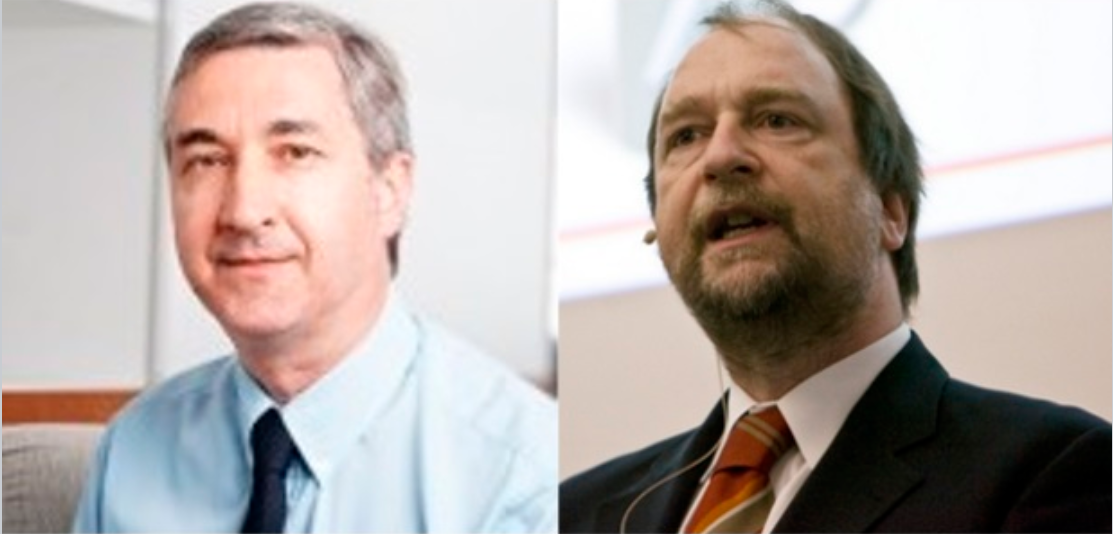
\includegraphics[height = 2cm]{./Imagenes/FidgeAndMattern.png}
        \end{center}
        
        Esta técnica consiste en un mapeo entre eventos en una
        historia distribuida y vectores enteros.
\end{frame}


\section{Algoritmo de Bhattacharya.} %%Título de la sección (Opcional)
\subsection{Introducción.}
\begin{frame}
  \frametitle{Motivación.}
  Observemos el siguiente caso partícular de polígono simple:
  
  \begin{center} 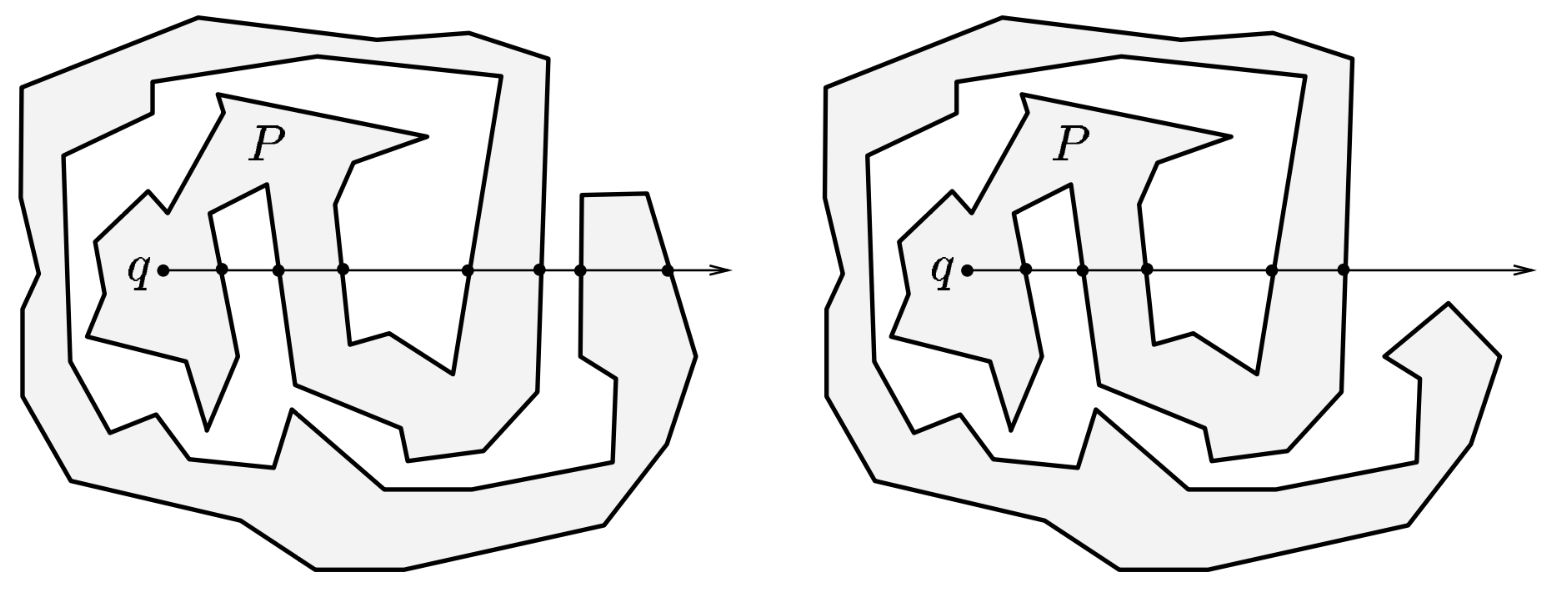
\includegraphics[width=0.55 \paperwidth]{images/Revoluciones.png} \end{center}

  El polígono de la izquierda tiene como número de revoluciones $2$ y el polígono
  de la derecha tiene cómo número de revoluciones $1$.
\end{frame}

\begin{frame}
  \frametitle{Poda de polígonos simples.}
  %\framesubtitle{Polígono de visibilidad.} %%Subtítulo de la diapositiva (opcional)
  Dado un polígono simple $P$ y un punto $q \in P$, calcular el polígono podado $P_1 \subseteq P$
  simple tal que $P_1$ contiene tanto a $V(q)$ como a $q$ y el número de revoluciones respecto de
  $q$ es a lo más $1$.  
\end{frame}

\subsection{Ejecución.}
% Estamos aquí ...
\begin{frame}
  \frametitle{Ejecución simple.}
  \centering 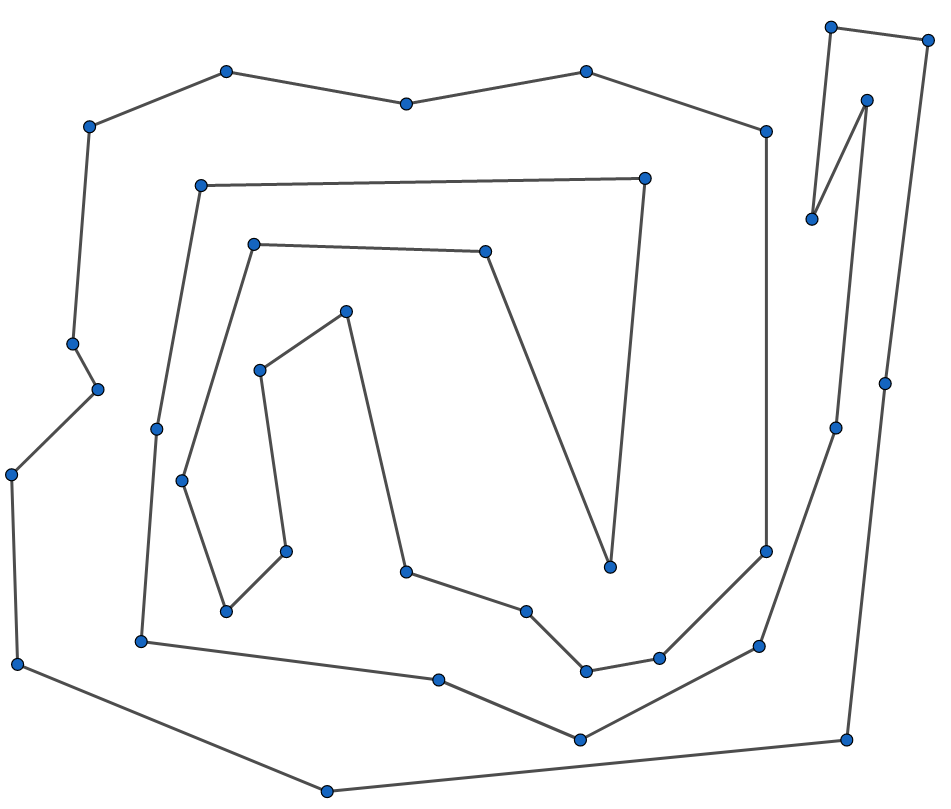
\includegraphics[width=0.45 \paperwidth]{images/Poda/1.png}
\end{frame}

\begin{frame}
  \centering 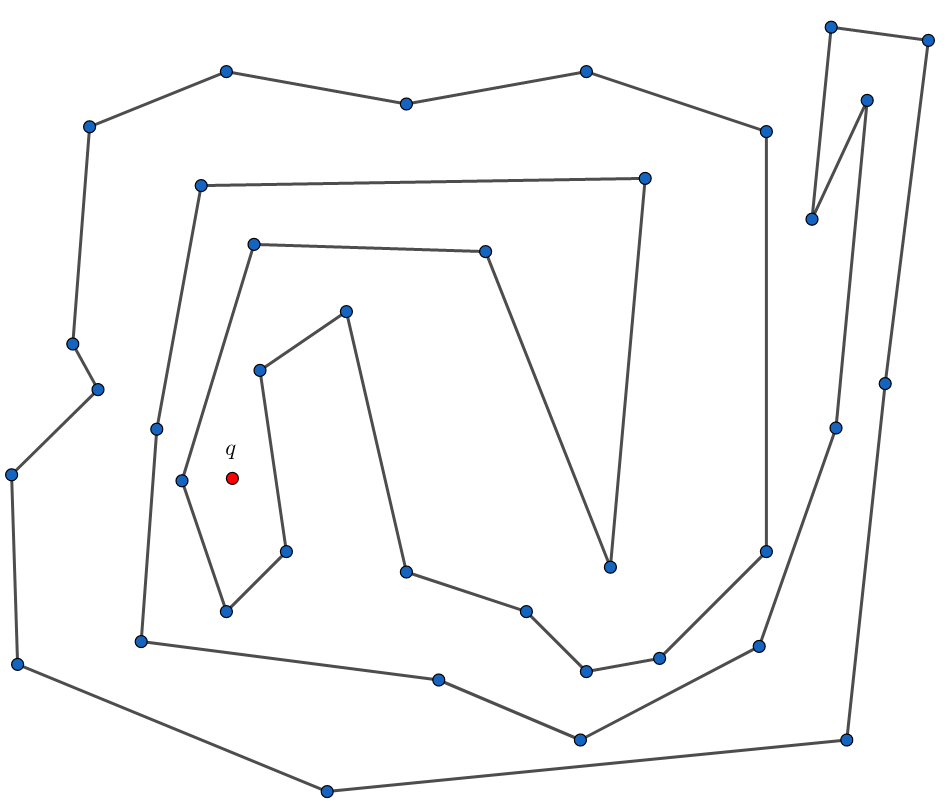
\includegraphics[width=0.45 \paperwidth]{images/Poda/2.png}
\end{frame}

\begin{frame}
  \centering 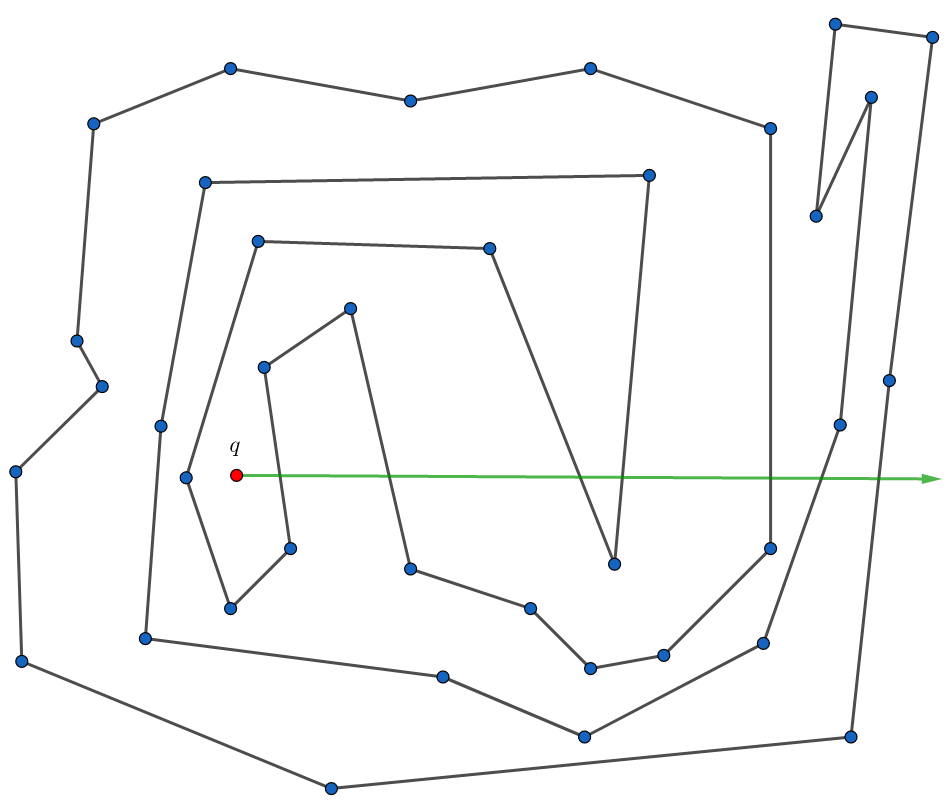
\includegraphics[width=0.45 \paperwidth]{images/Poda/3.png}
\end{frame}

\begin{frame}
  \centering 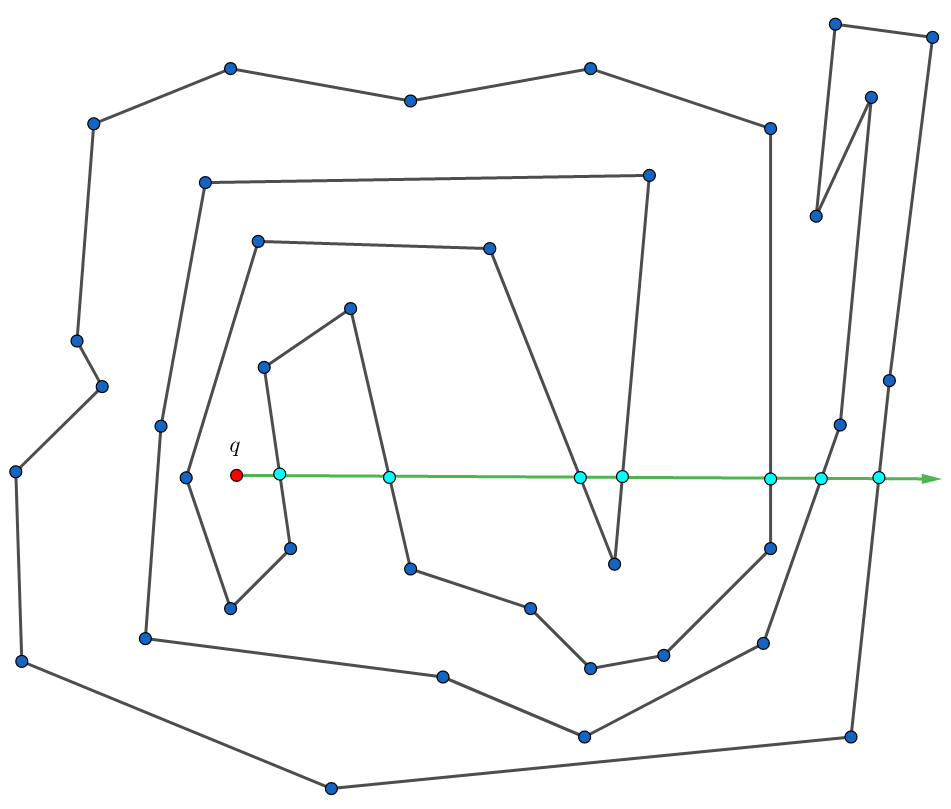
\includegraphics[width=0.45 \paperwidth]{images/Poda/4.png}
\end{frame}

\begin{frame}
  \centering 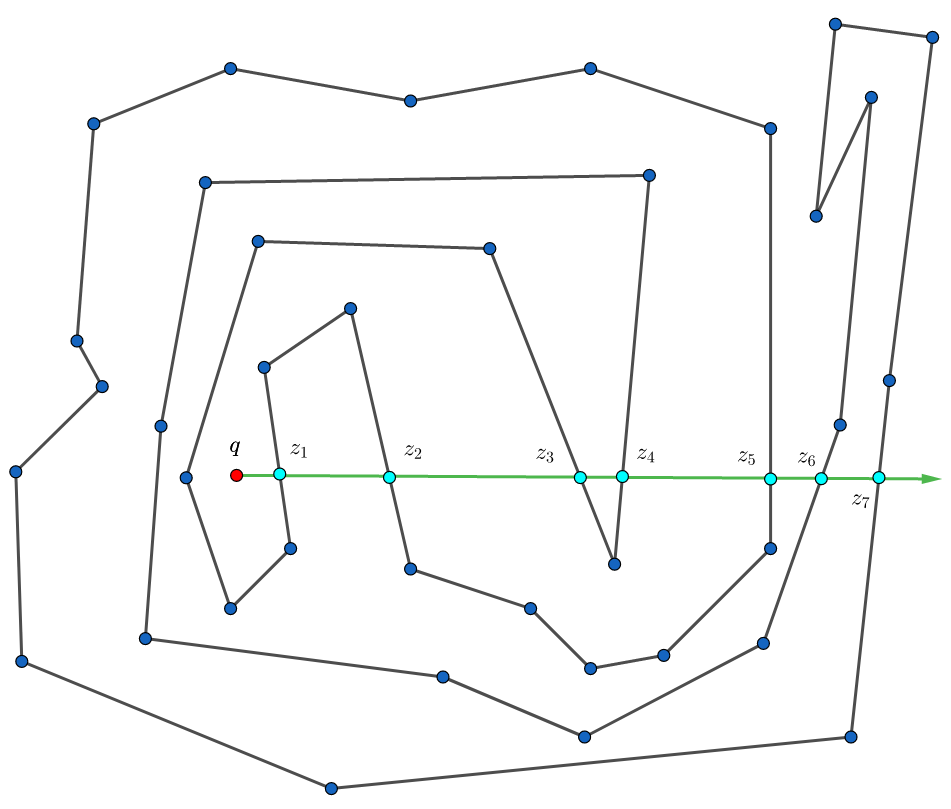
\includegraphics[width=0.45 \paperwidth]{images/Poda/5.png}
\end{frame}

\begin{frame}
  \centering 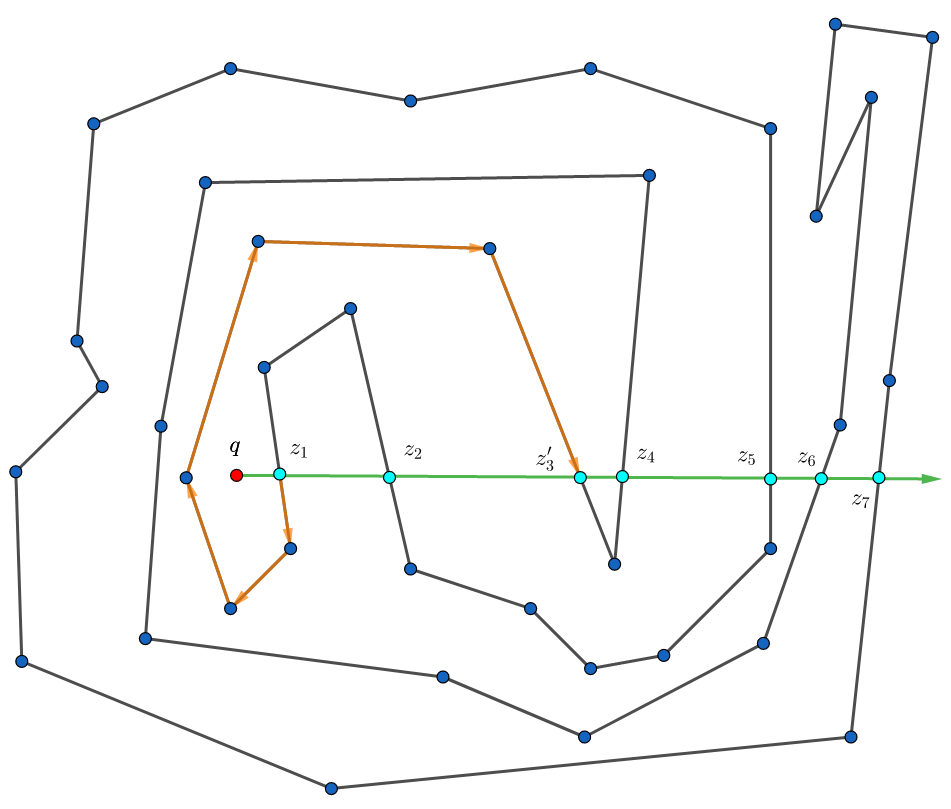
\includegraphics[width=0.45 \paperwidth]{images/Poda/6.png}
\end{frame}

\begin{frame}
  \centering 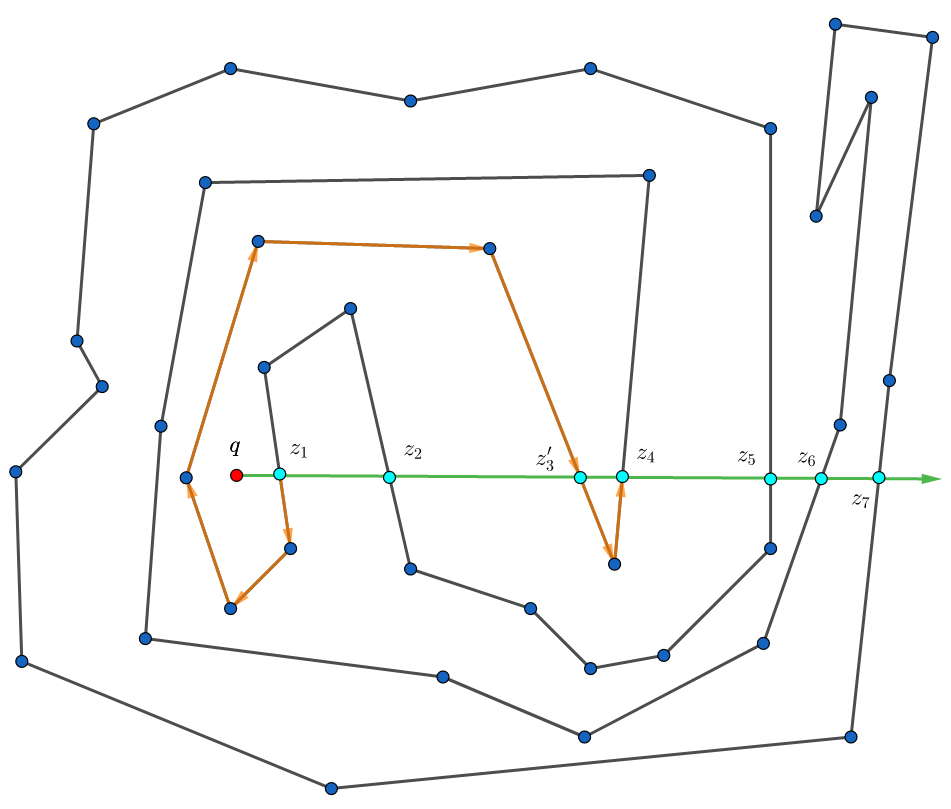
\includegraphics[width=0.45 \paperwidth]{images/Poda/7.png}
\end{frame}

\begin{frame}
  \centering 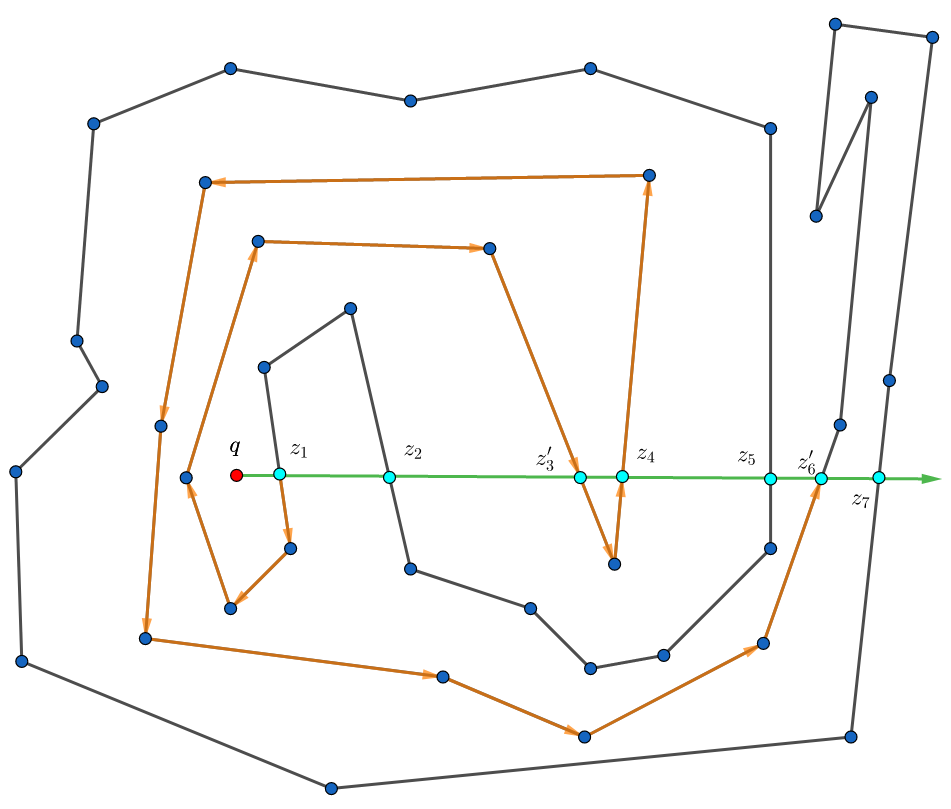
\includegraphics[width=0.45 \paperwidth]{images/Poda/8.png}
\end{frame}

\begin{frame}
  \centering 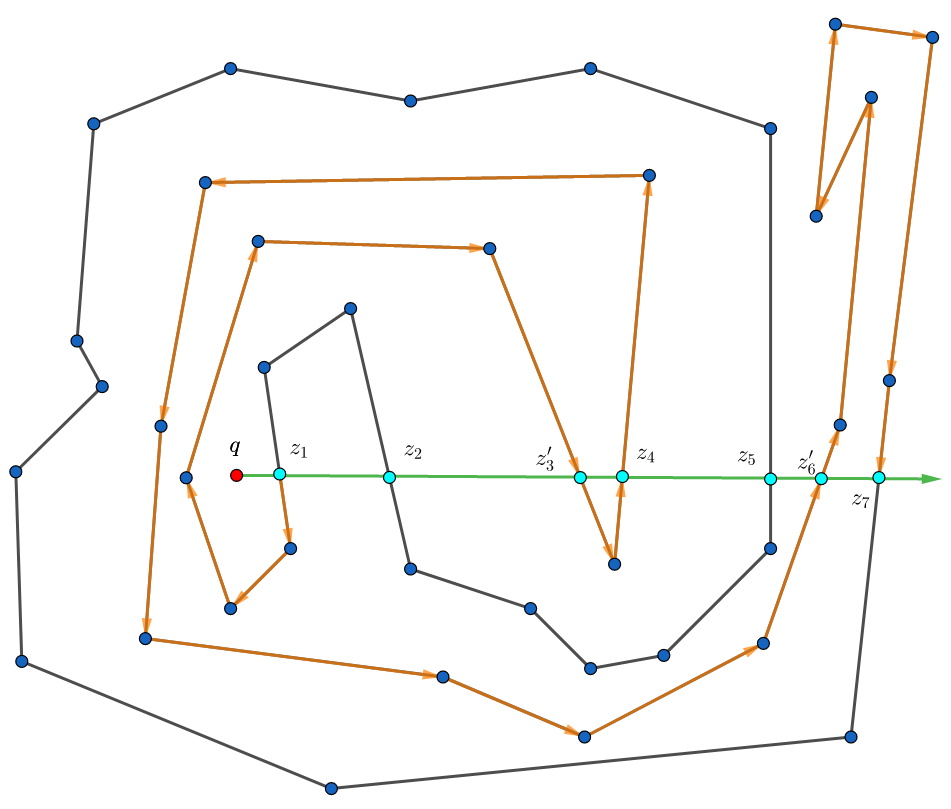
\includegraphics[width=0.45 \paperwidth]{images/Poda/9.png}
\end{frame}

\begin{frame}
  \centering 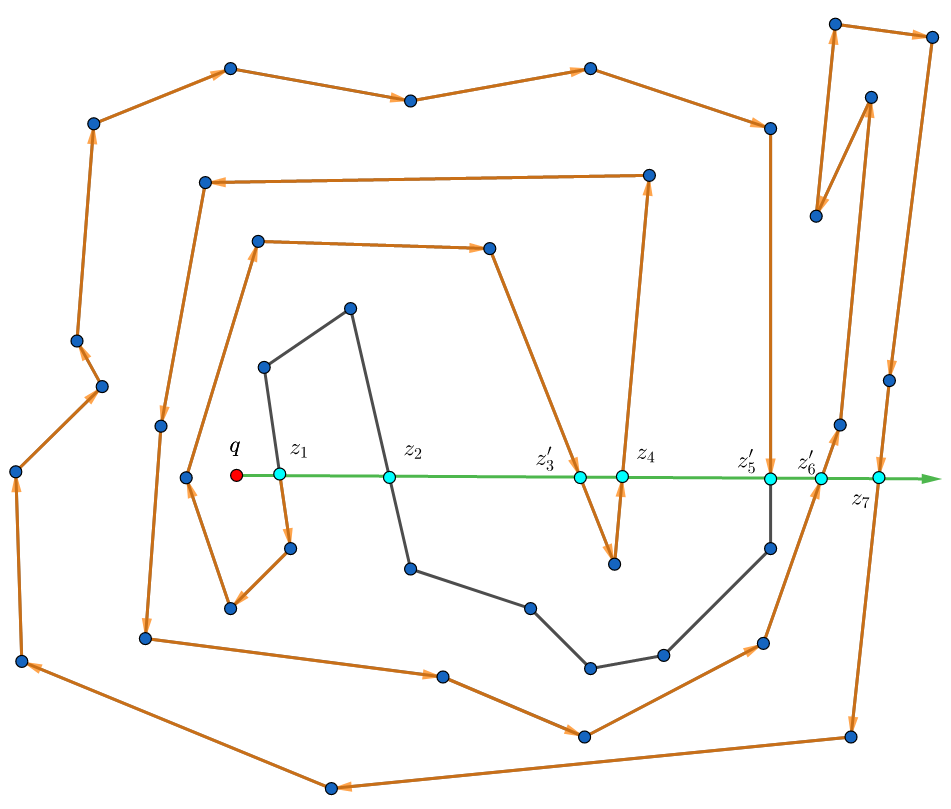
\includegraphics[width=0.45 \paperwidth]{images/Poda/10.png}
\end{frame}

\begin{frame}
  \centering 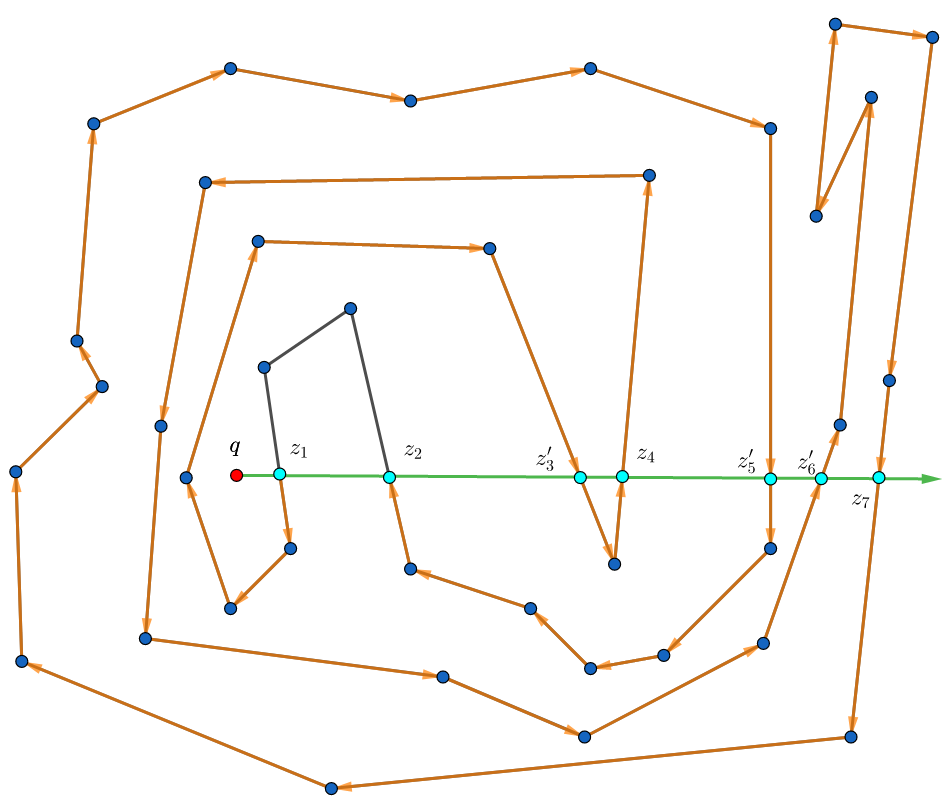
\includegraphics[width=0.45 \paperwidth]{images/Poda/11.png}
\end{frame}

\begin{frame}
  \centering 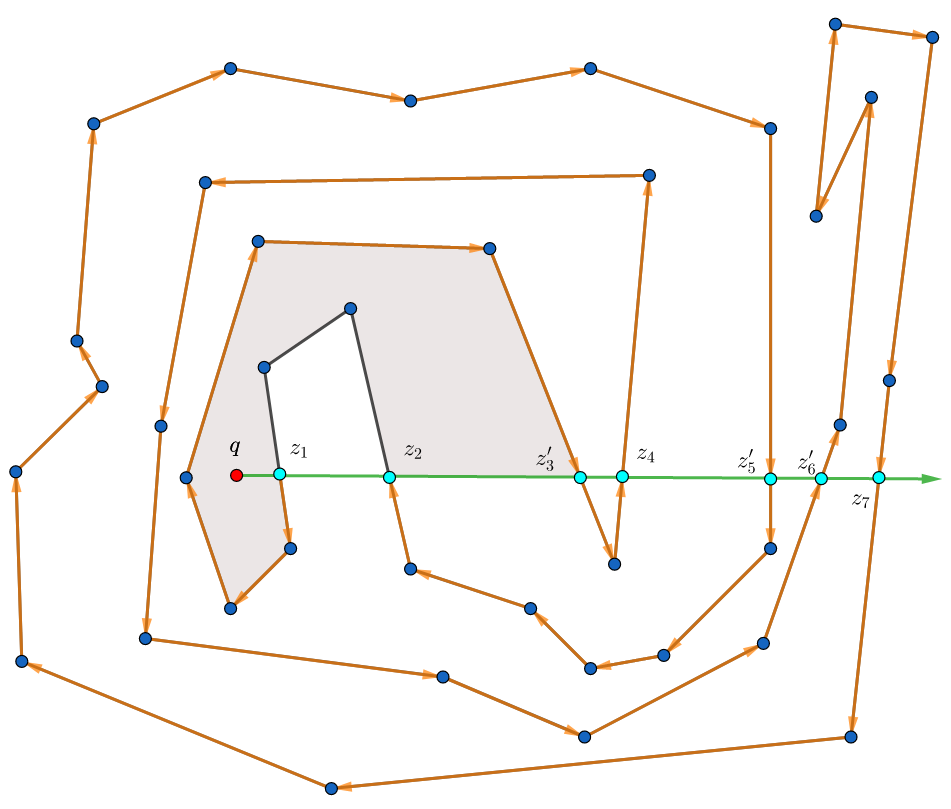
\includegraphics[width=0.45 \paperwidth]{images/Poda/12.png}
\end{frame}
\subsection{Análisis de complejidad.}

\begin{frame}
  \frametitle{Análisis de la complejidad.}
  \begin{enumerate}
  \item Lanzar el rayo lo hacemos en tiempo constante.
  \item Encontrar el primer punto que intersecta la frontera lo hacemos en $\mathcal{O}(\log n)$
    por medio de una búsqueda en las aristas de $P$.
  \item Clasificar las intersecciones lo hacemos en $\mathcal{O}(n)$, pues debemos recorrer el
    polígono $P$.
  \item Encontrar la primer arista respecto a $q$ tal que tenga sus dos extremos clasificados con
    diferente denominación $\{\text{abajo}, \text{ arriba}\}$ lo realizamos en $\mathcal{O}(n)$
    al recorrer nuevamente nuestro polígono.
  \end{enumerate}
\end{frame}


\section{Algoritmo de Lee.} %%Título de la sección (Opcional)
\subsection{Introducción.}
\begin{frame}
  \frametitle{Motivación.}
  Queremos obtener el polígono de visibilidad $V(q)$ dado un punto $q$ y un polígono
  simple $P$.\newline

  \textbf{Obs.} Si
  \[V(q) = P,\]
  entonces $P$ es un polígono estrellado.\newline

  Asumimos que el polígono a trabajar no tiene un número de revoluciones mayor a $1$.
\end{frame}

\subsection{Ejecución.}
\begin{frame}
  \centering 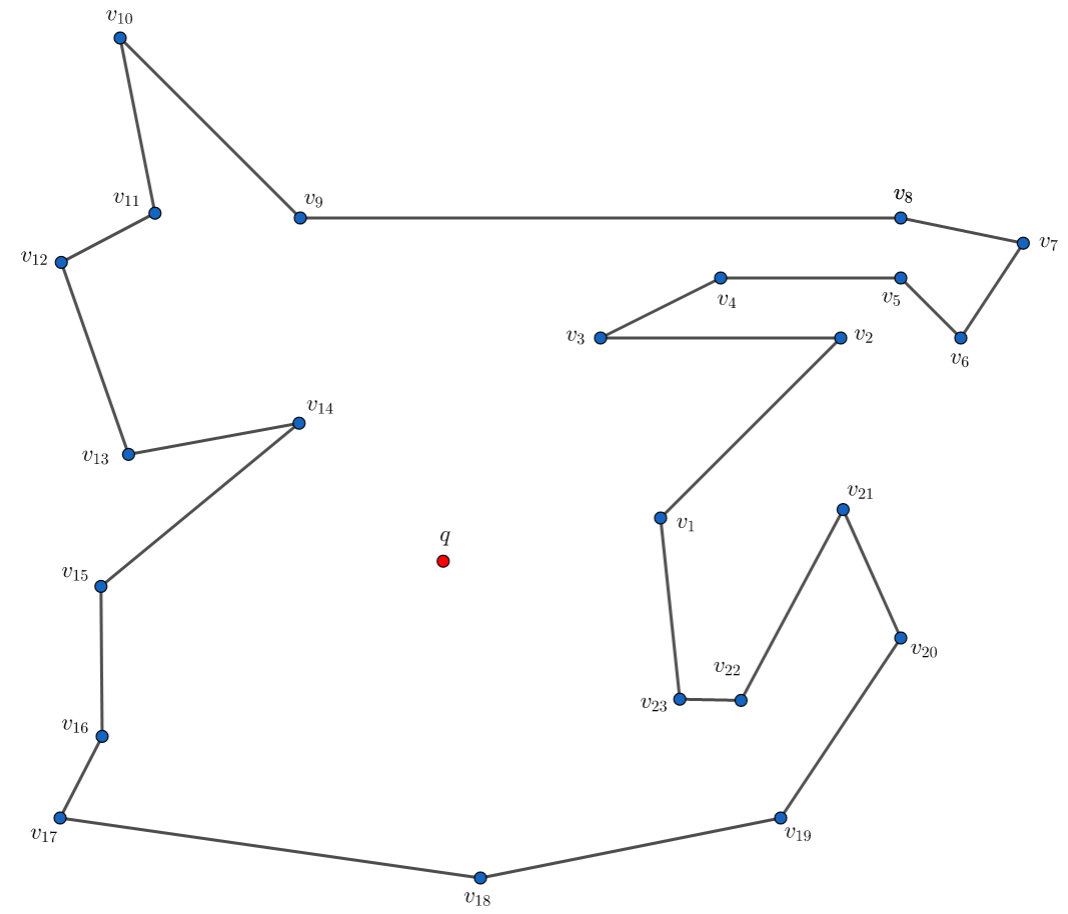
\includegraphics[width=0.70 \paperwidth]{images/Ejecucion/e01.png}
\end{frame}

\begin{frame}
  \centering 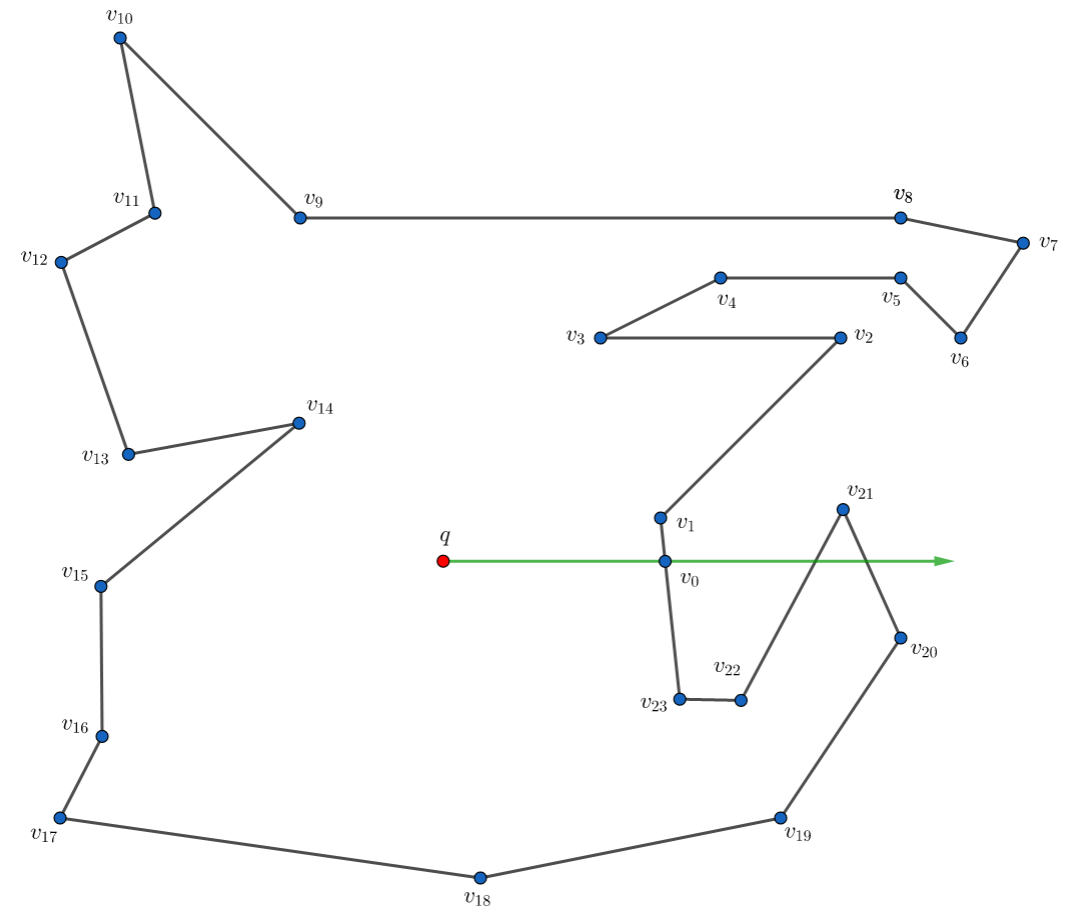
\includegraphics[width=0.70 \paperwidth]{images/Ejecucion/e02.png}
\end{frame}

\begin{frame}
  \centering 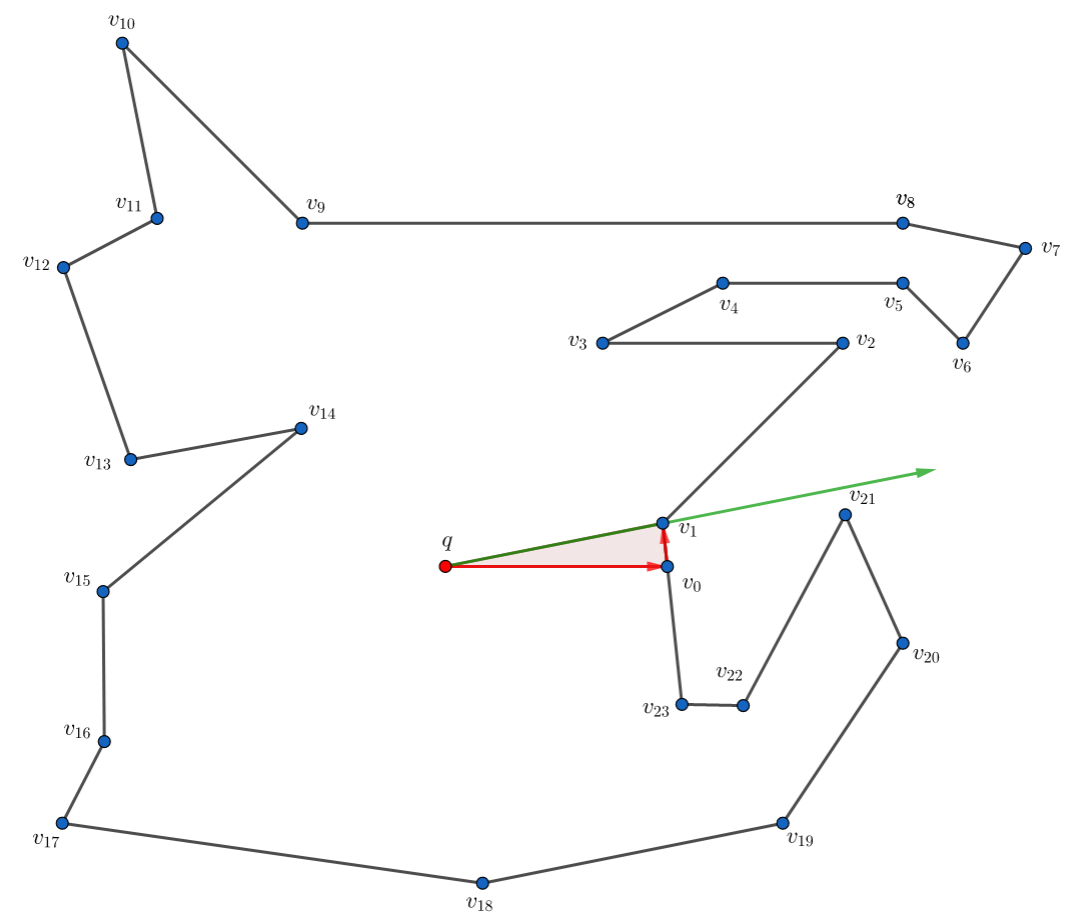
\includegraphics[width=0.70 \paperwidth]{images/Ejecucion/e03.png}
\end{frame}

\begin{frame}
  \centering 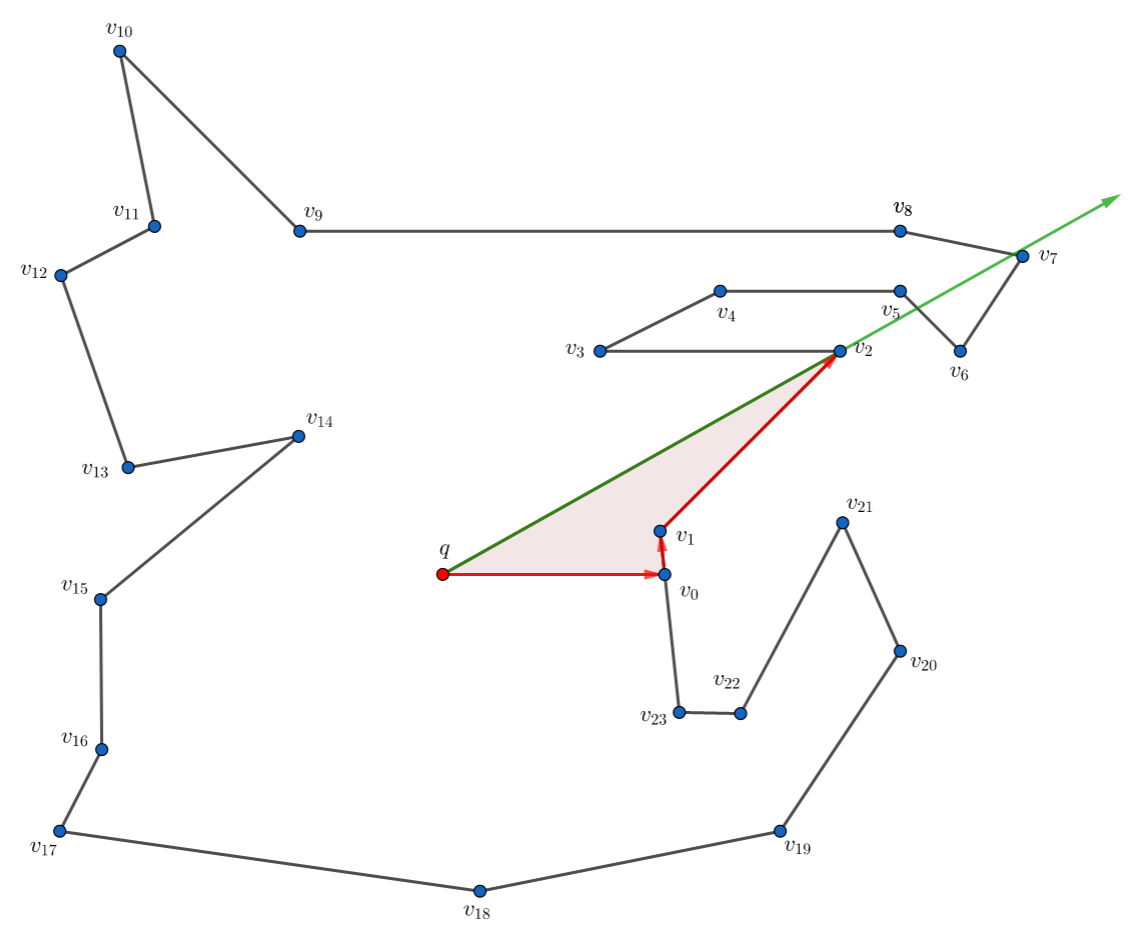
\includegraphics[width=0.70 \paperwidth]{images/Ejecucion/e04.png}
\end{frame}

\begin{frame}
  \centering 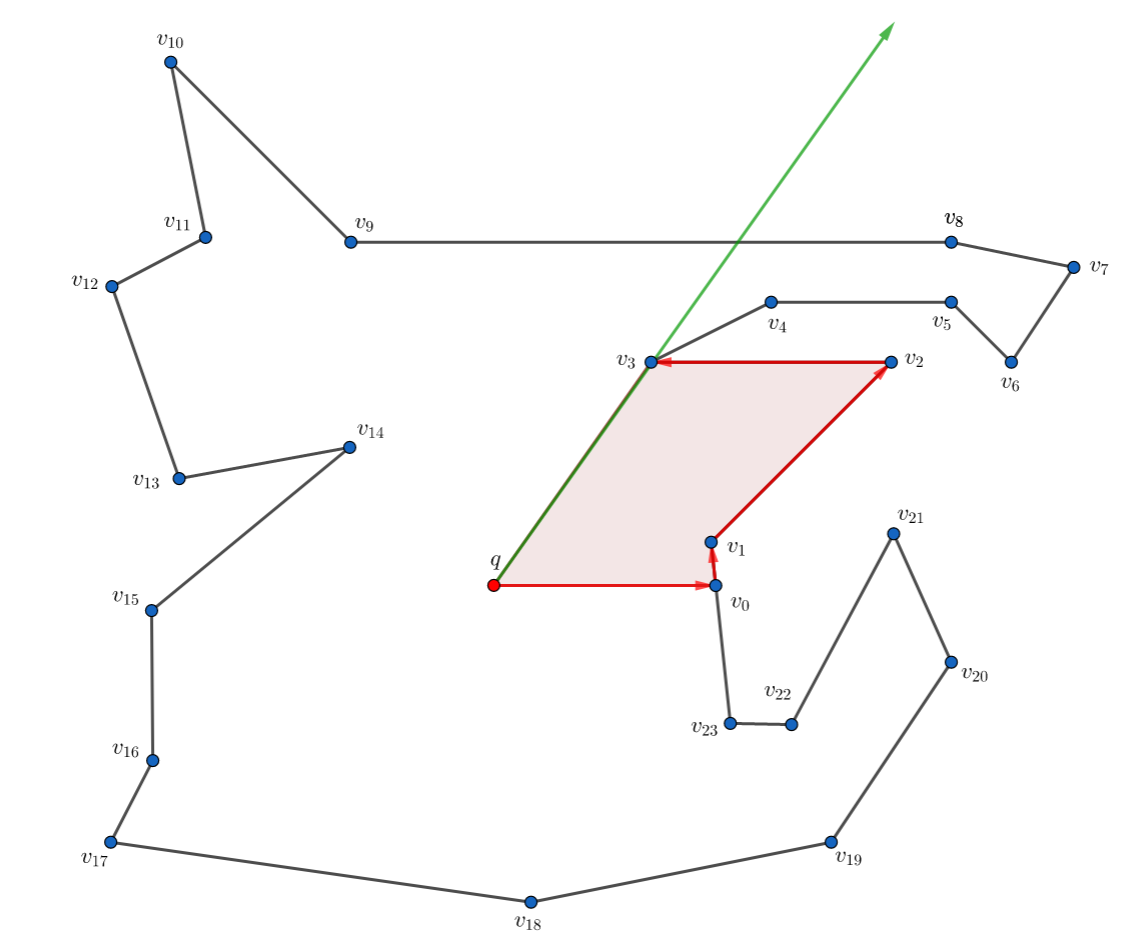
\includegraphics[width=0.70 \paperwidth]{images/Ejecucion/e05.png}
\end{frame}

\begin{frame}
  \centering 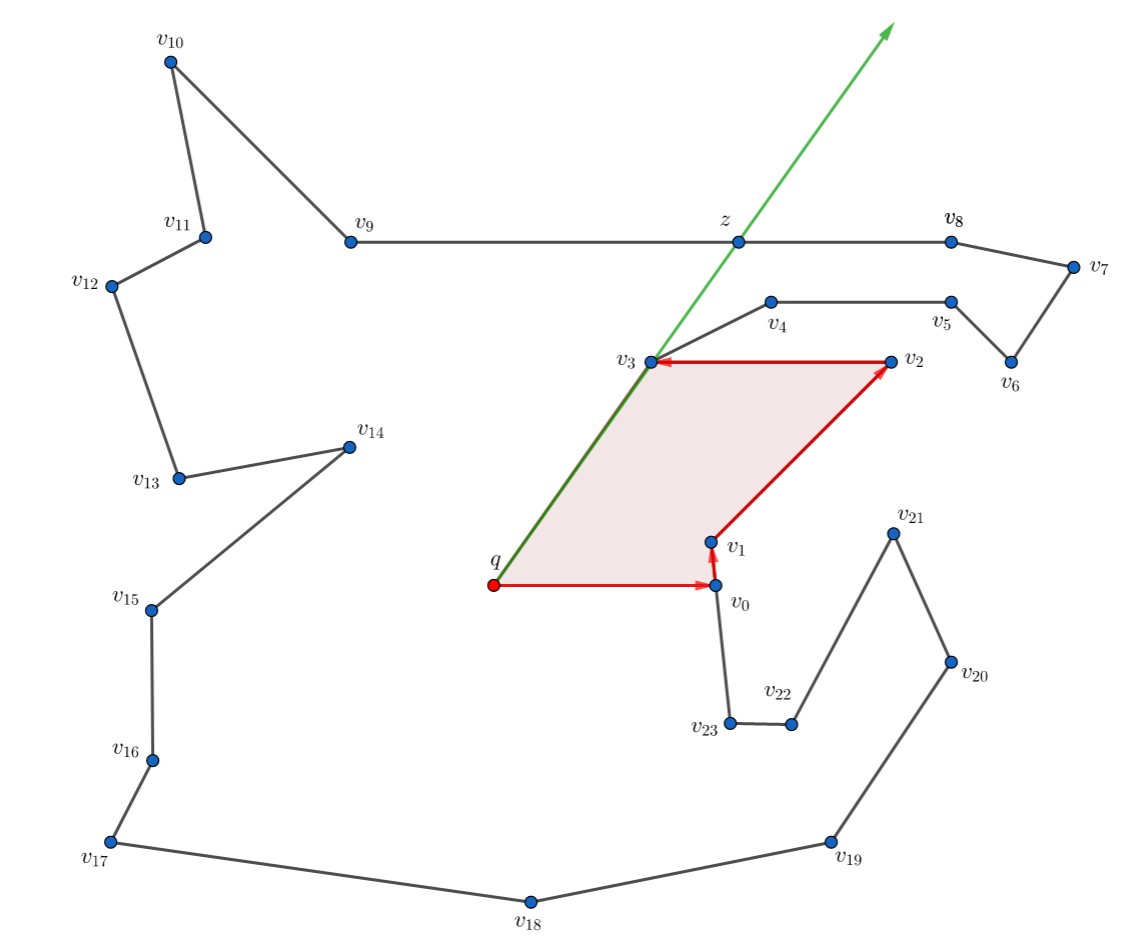
\includegraphics[width=0.70 \paperwidth]{images/Ejecucion/e06.png}
\end{frame}

\begin{frame}
  \centering 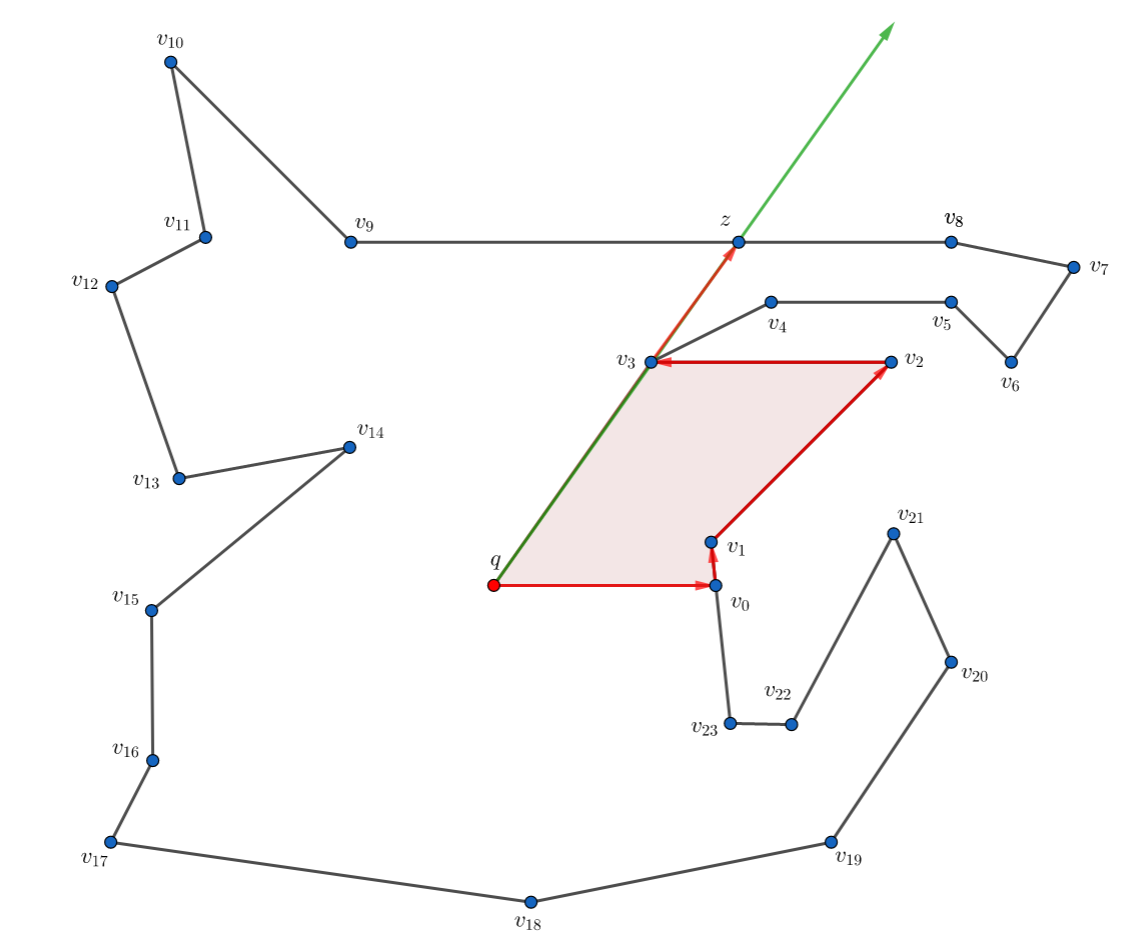
\includegraphics[width=0.70 \paperwidth]{images/Ejecucion/e07.png}
\end{frame}

\begin{frame}
  \centering 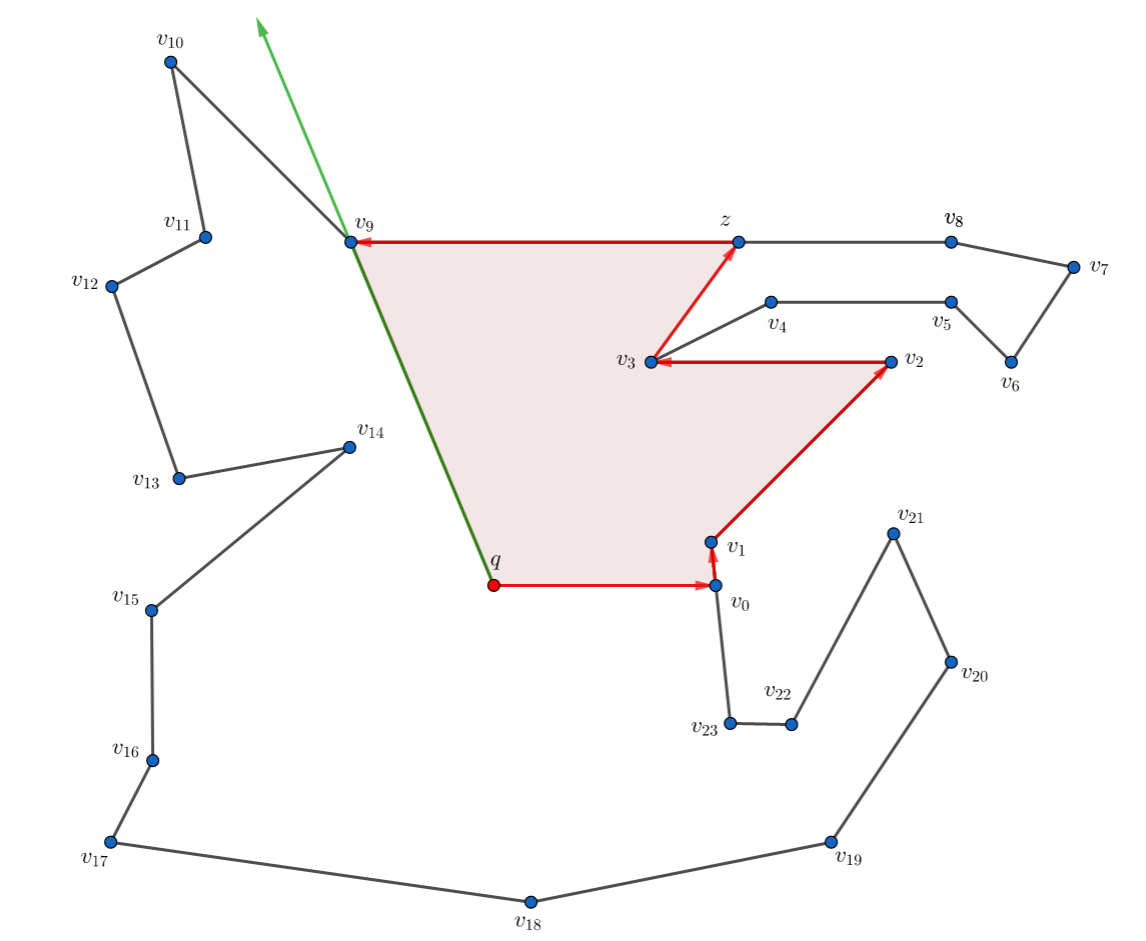
\includegraphics[width=0.70 \paperwidth]{images/Ejecucion/e08.png}
\end{frame}

\begin{frame}
  \centering 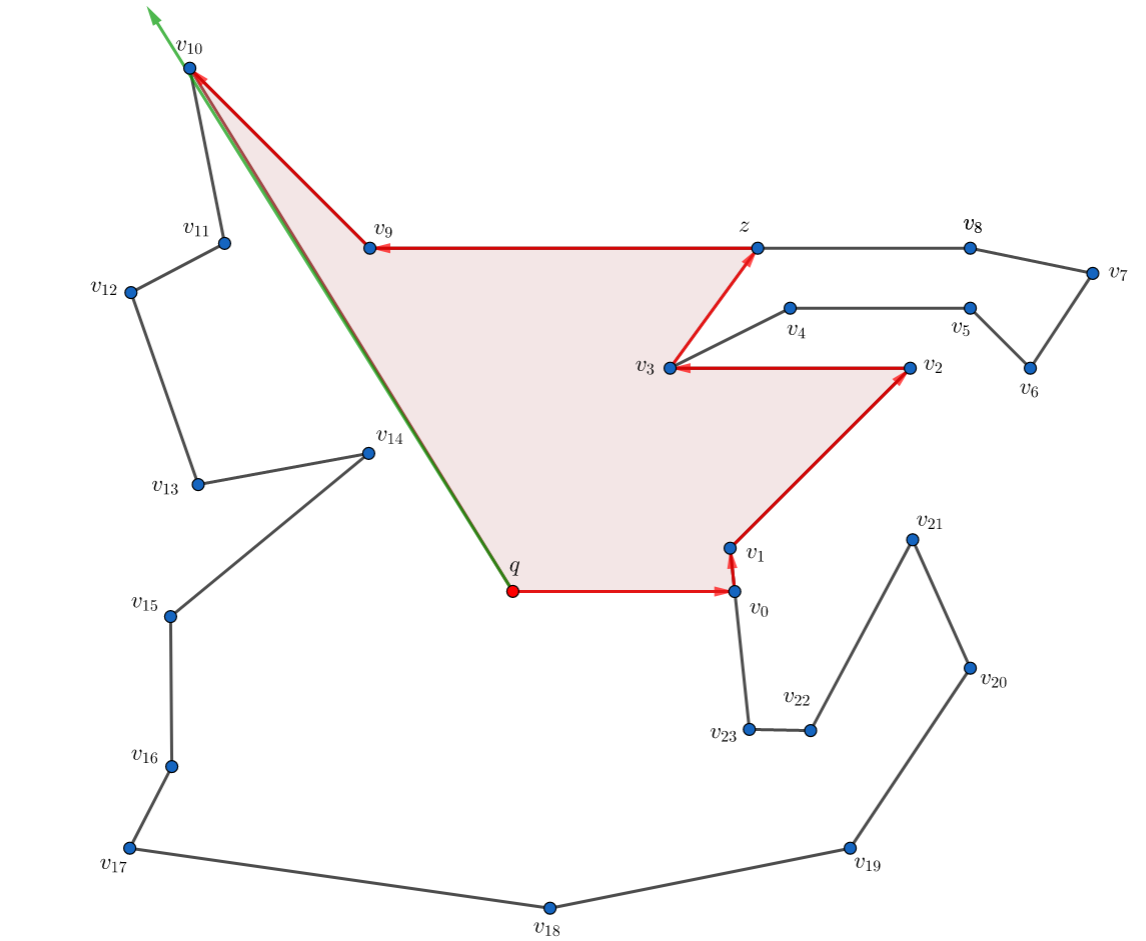
\includegraphics[width=0.70 \paperwidth]{images/Ejecucion/e09.png}
\end{frame}

\begin{frame}
  \centering 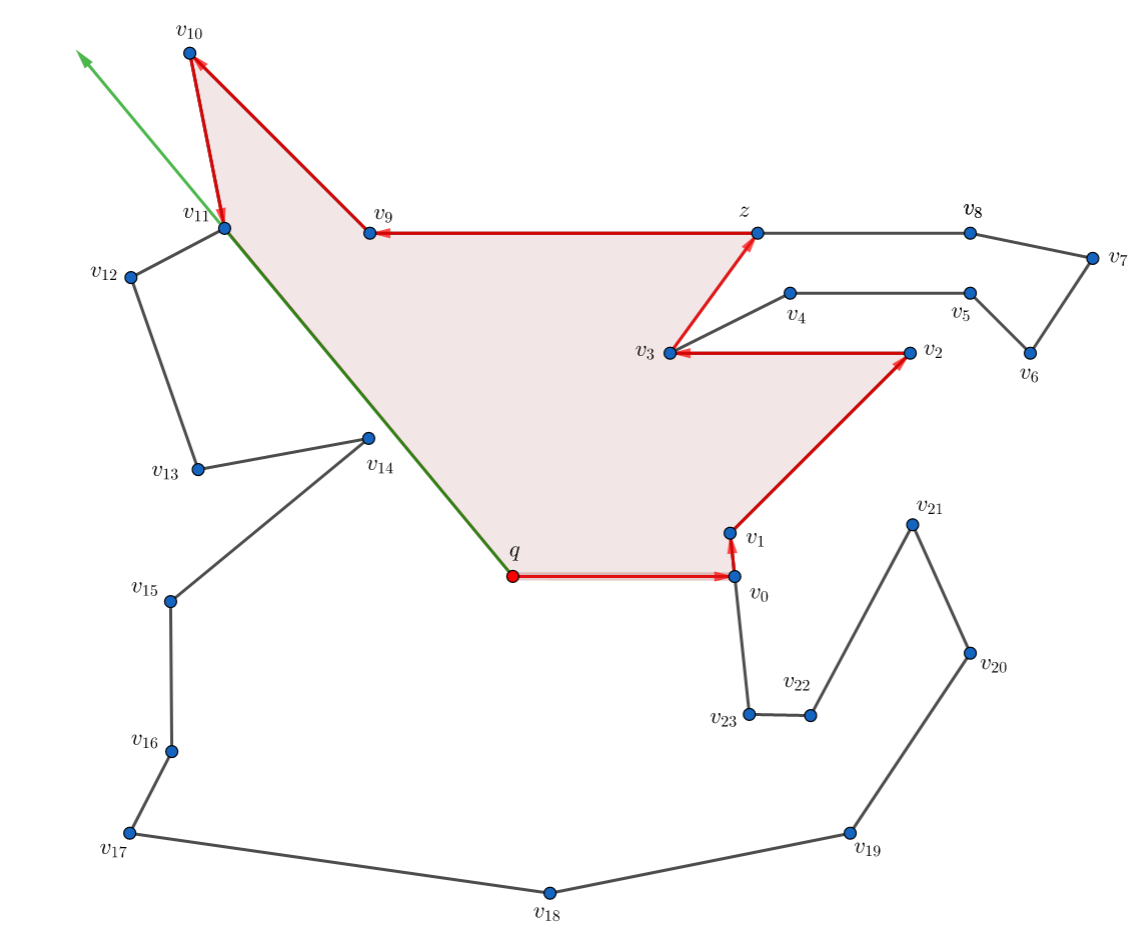
\includegraphics[width=0.70 \paperwidth]{images/Ejecucion/e10.png}
\end{frame}

\begin{frame}
  \centering 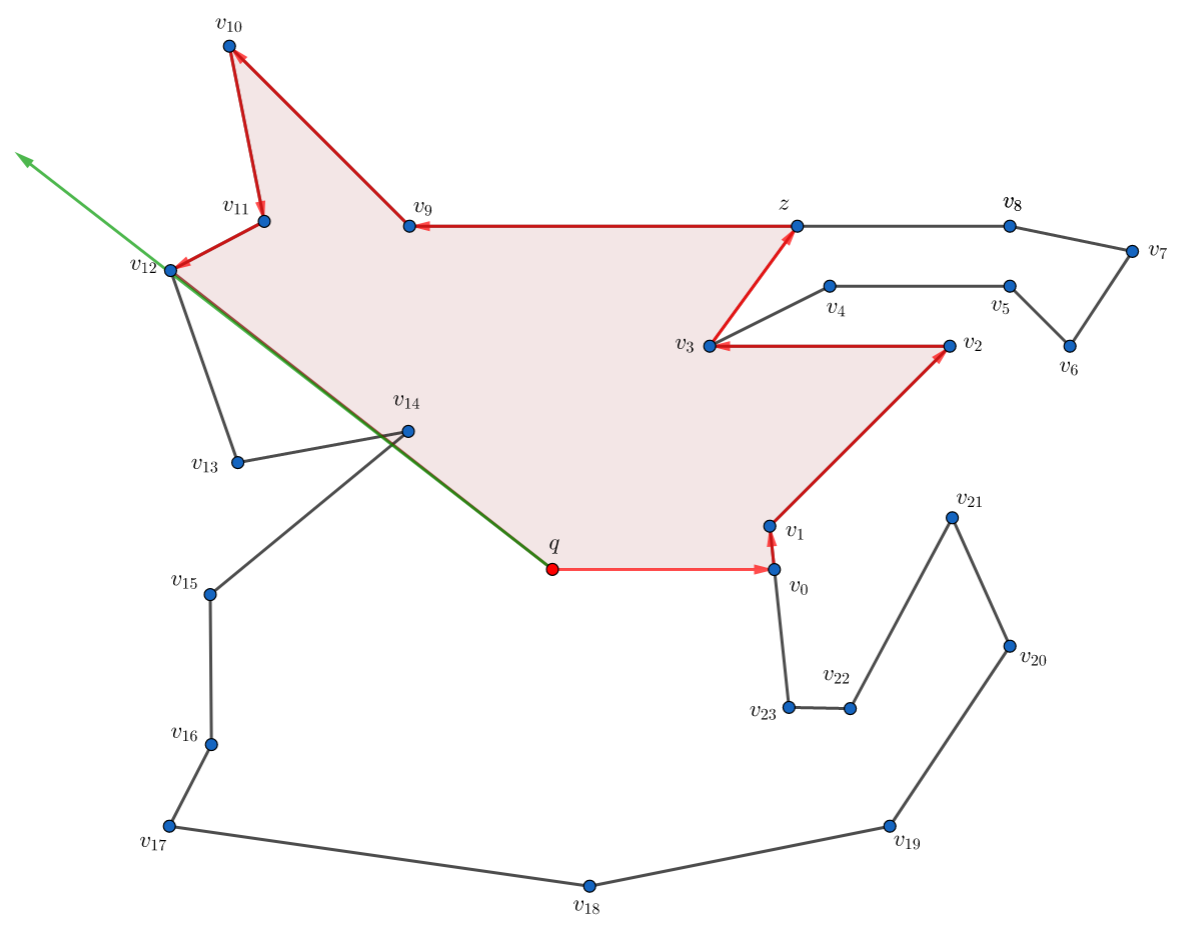
\includegraphics[width=0.70 \paperwidth]{images/Ejecucion/e11.png}
\end{frame}

\begin{frame}
  \centering 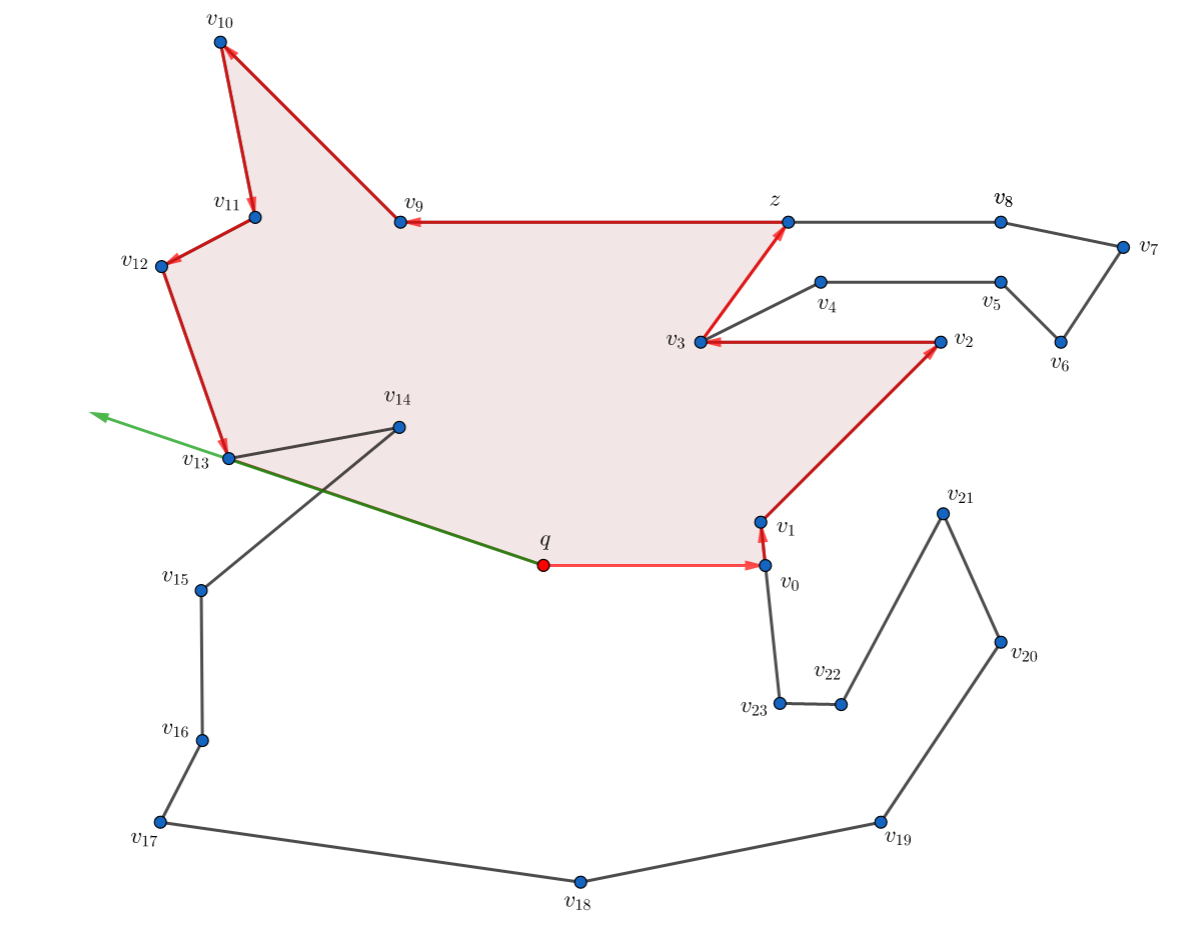
\includegraphics[width=0.70 \paperwidth]{images/Ejecucion/e12.png}
\end{frame}

\begin{frame}
  \centering 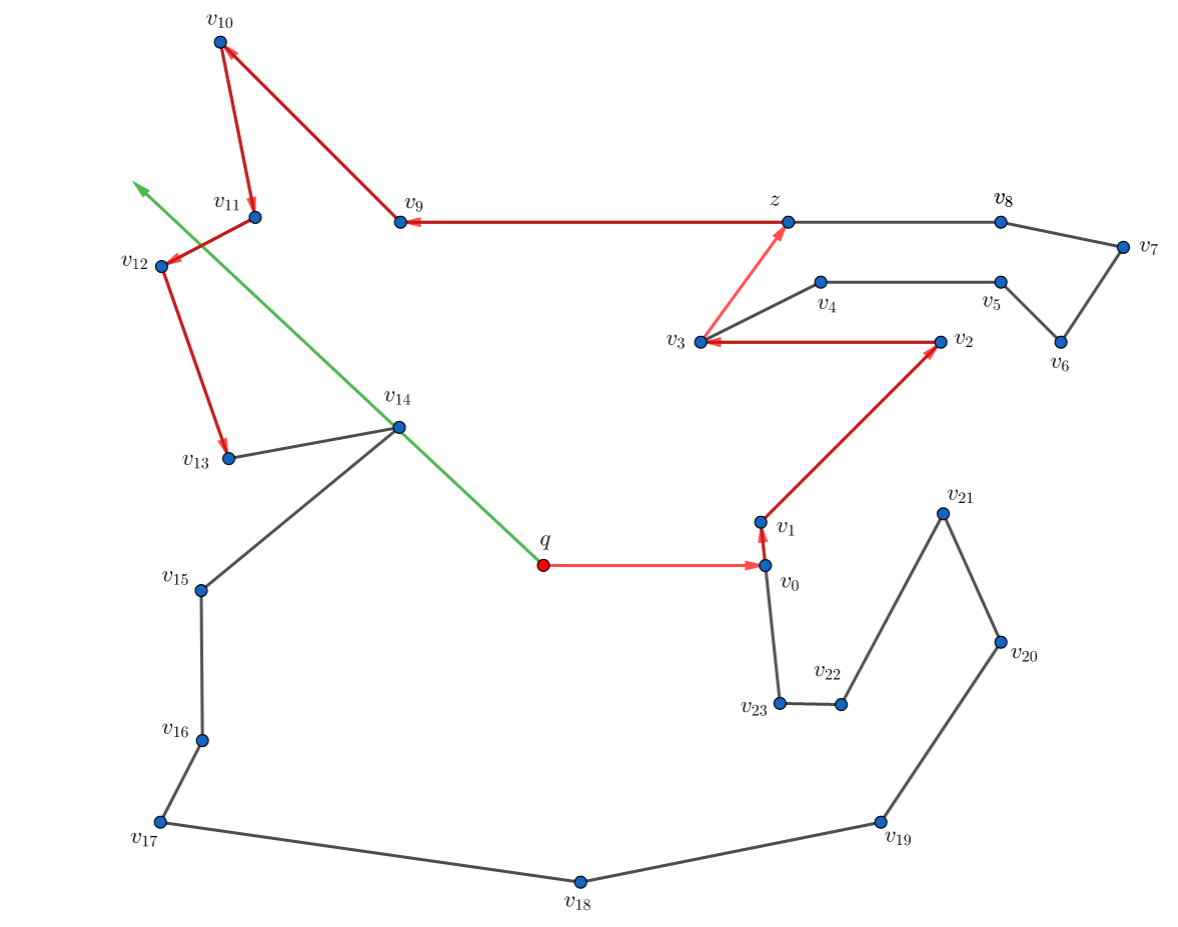
\includegraphics[width=0.70 \paperwidth]{images/Ejecucion/e13.png}
\end{frame}

\begin{frame}
  \centering 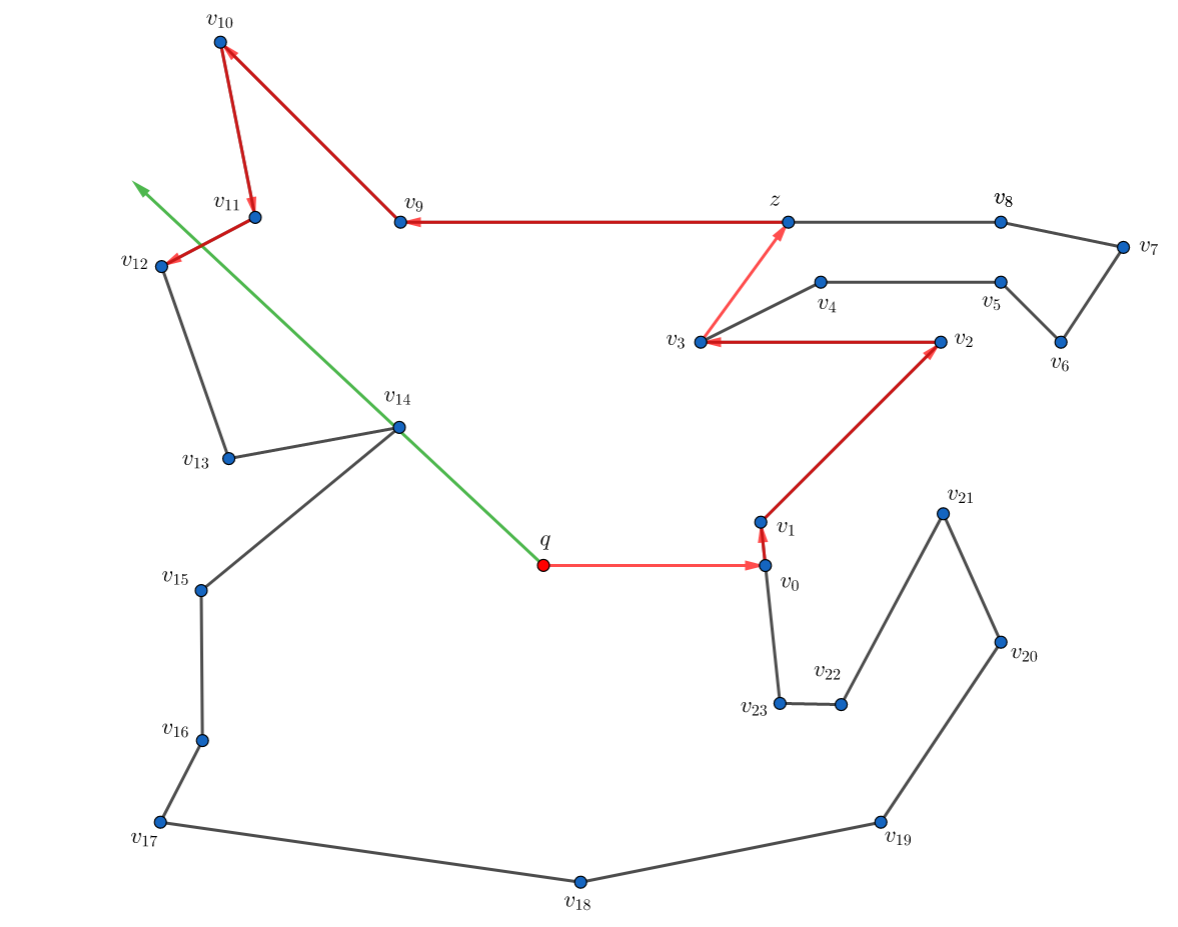
\includegraphics[width=0.70 \paperwidth]{images/Ejecucion/e14.png}
\end{frame}

\begin{frame}
  \centering 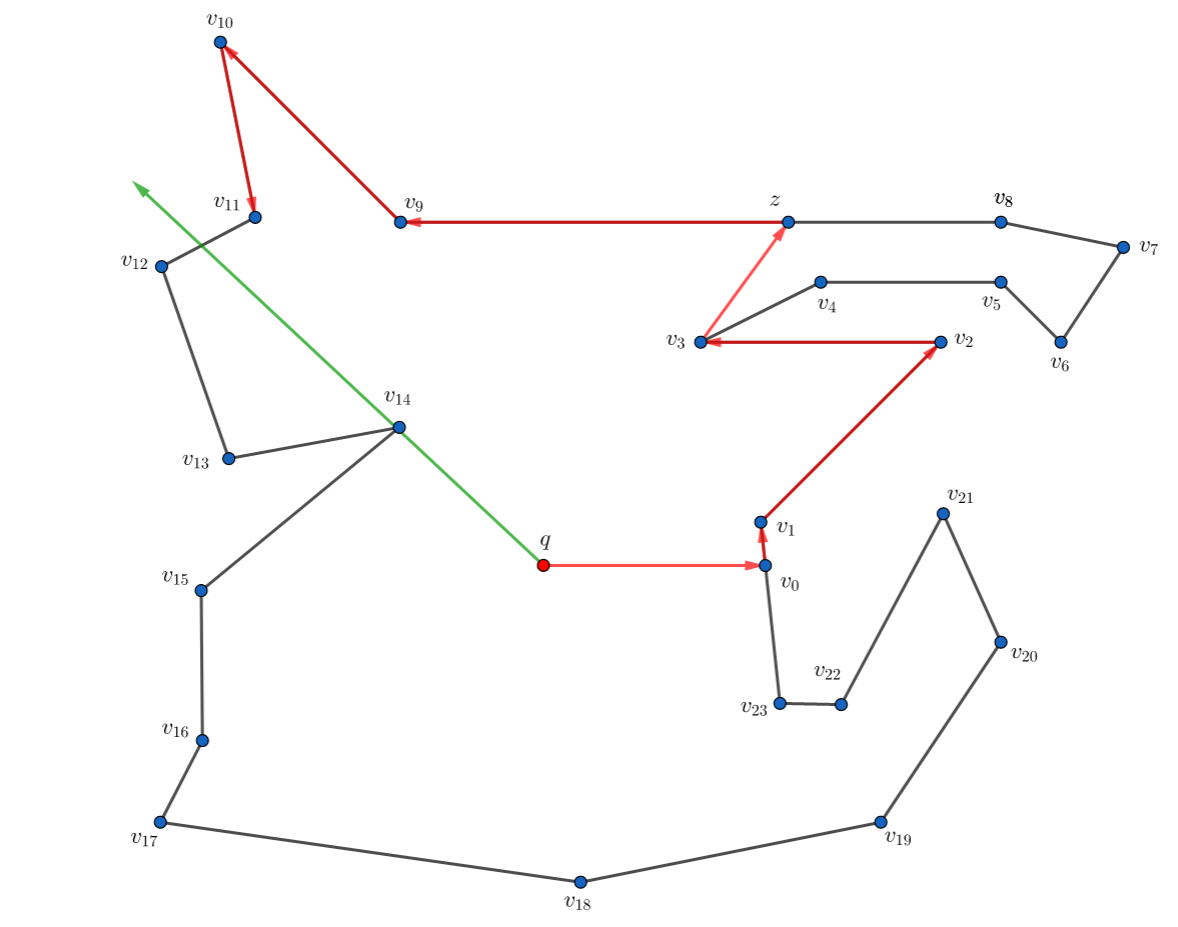
\includegraphics[width=0.70 \paperwidth]{images/Ejecucion/e15.png}
\end{frame}

\begin{frame}
  \centering 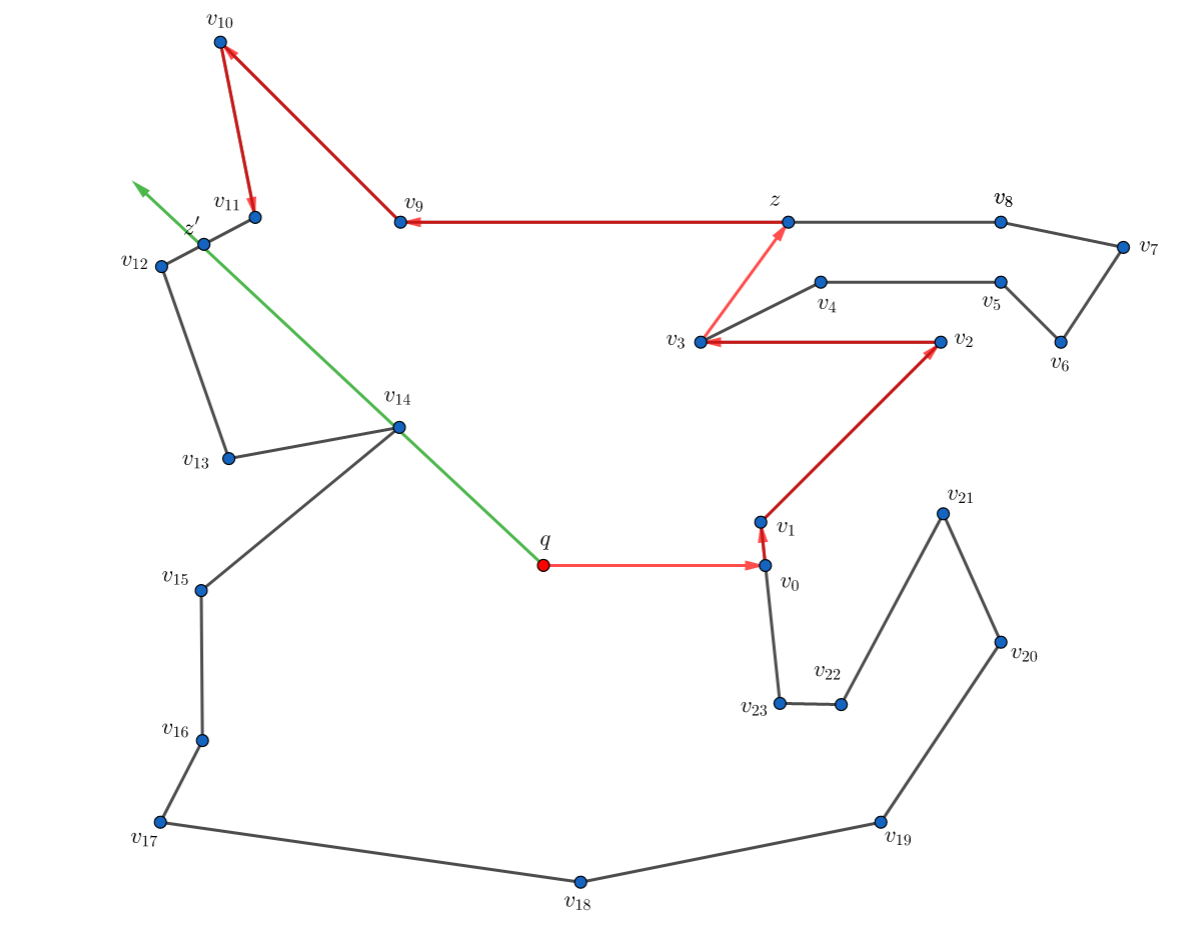
\includegraphics[width=0.70 \paperwidth]{images/Ejecucion/e16.png}
\end{frame}

\begin{frame}
  \centering 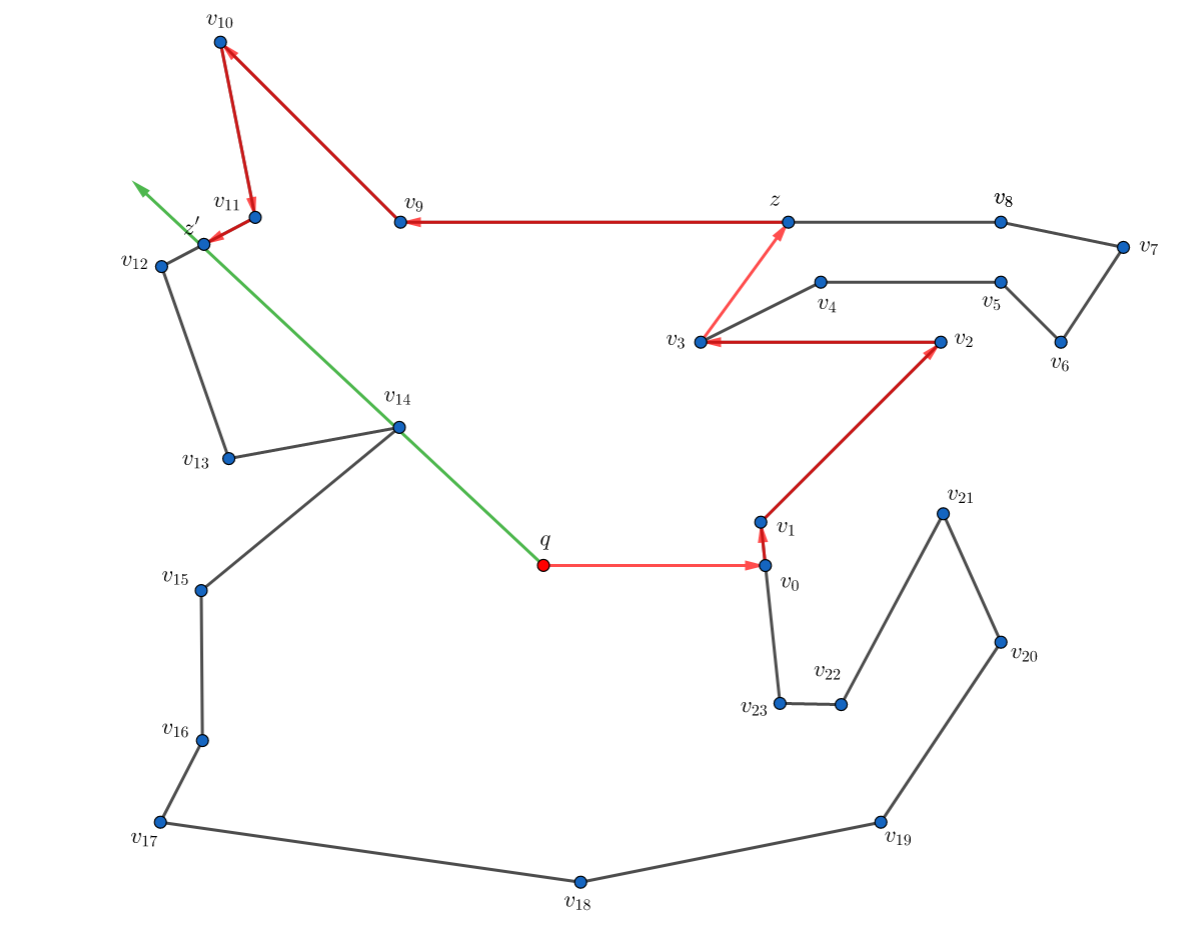
\includegraphics[width=0.70 \paperwidth]{images/Ejecucion/e17.png}
\end{frame}

\begin{frame}
  \centering 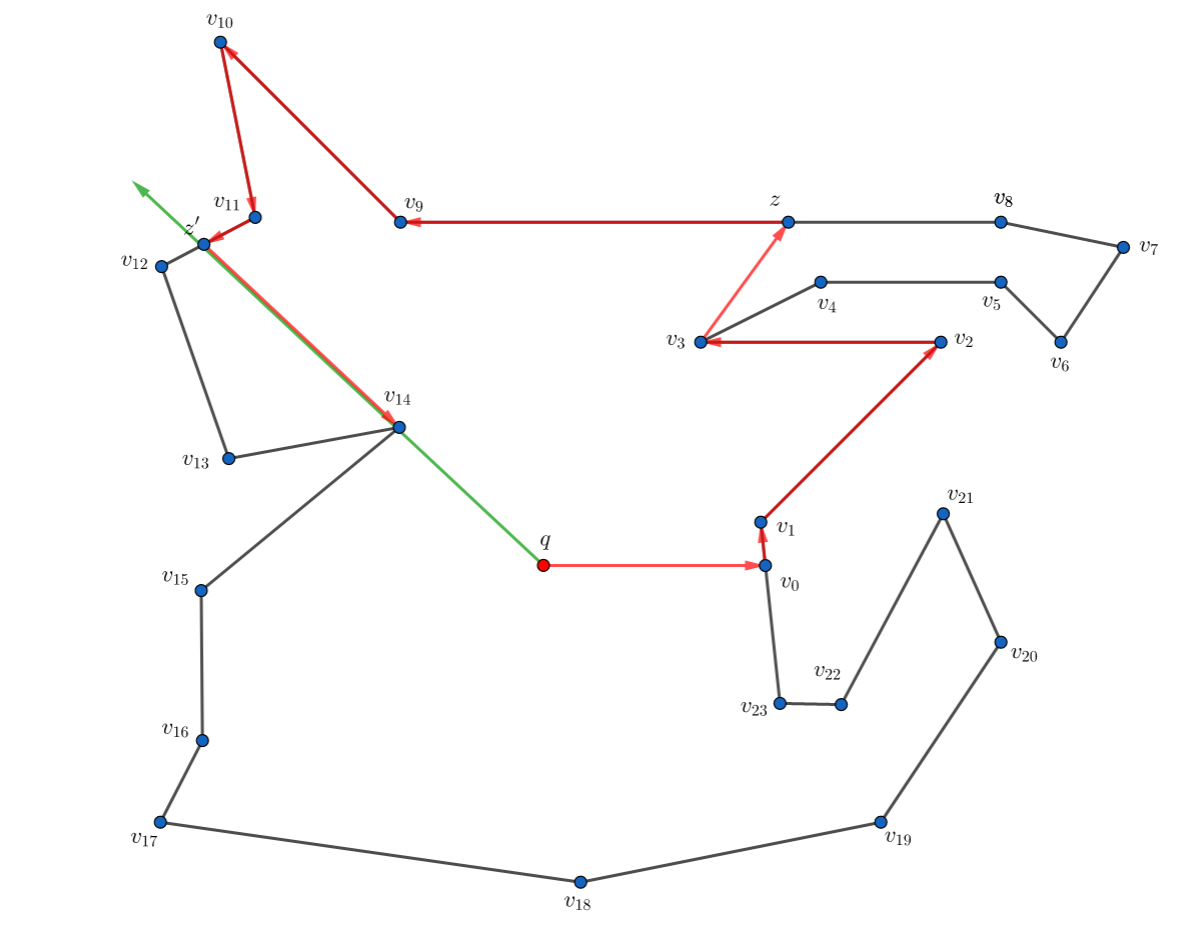
\includegraphics[width=0.70 \paperwidth]{images/Ejecucion/e18.png}
\end{frame}

\begin{frame}
  \centering 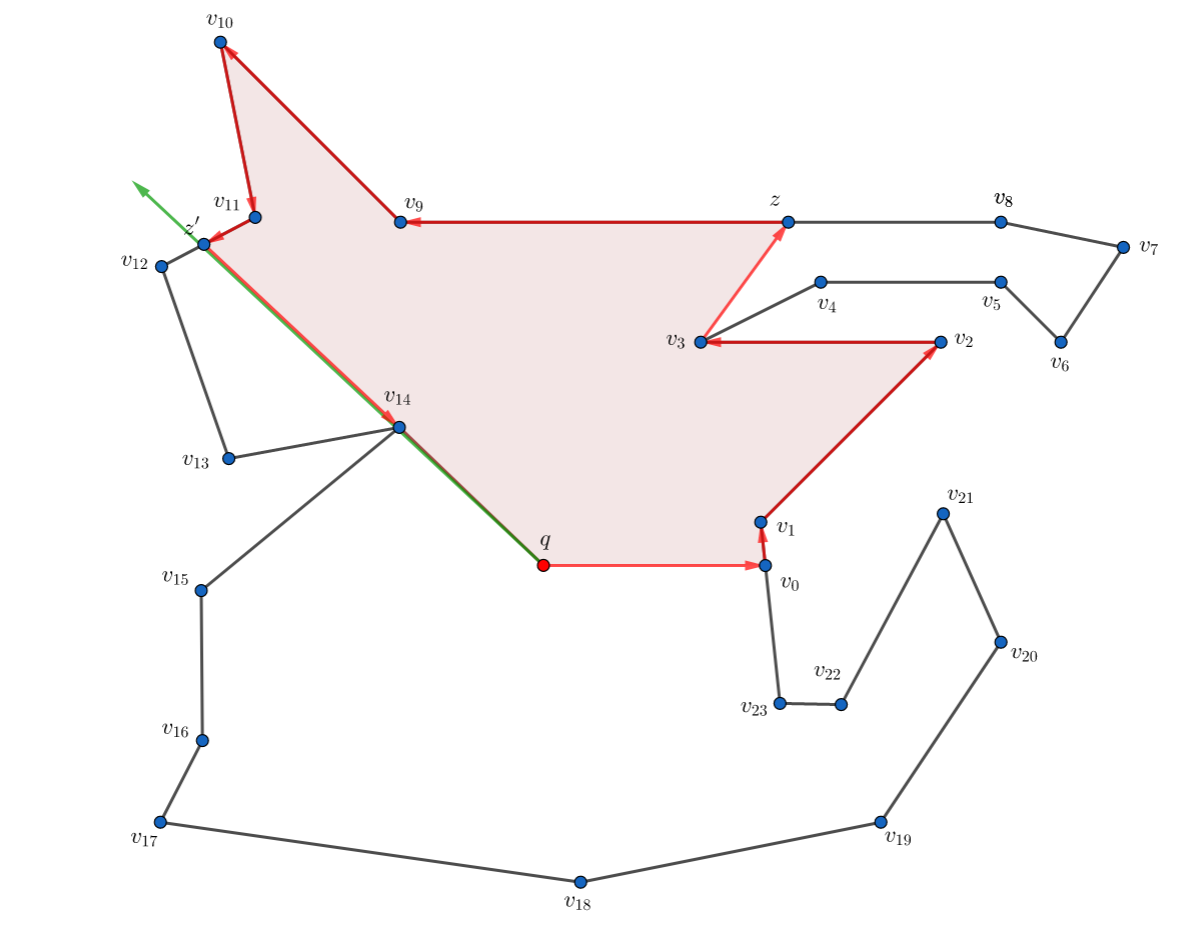
\includegraphics[width=0.70 \paperwidth]{images/Ejecucion/e19.png}
\end{frame}

\begin{frame}
  \centering 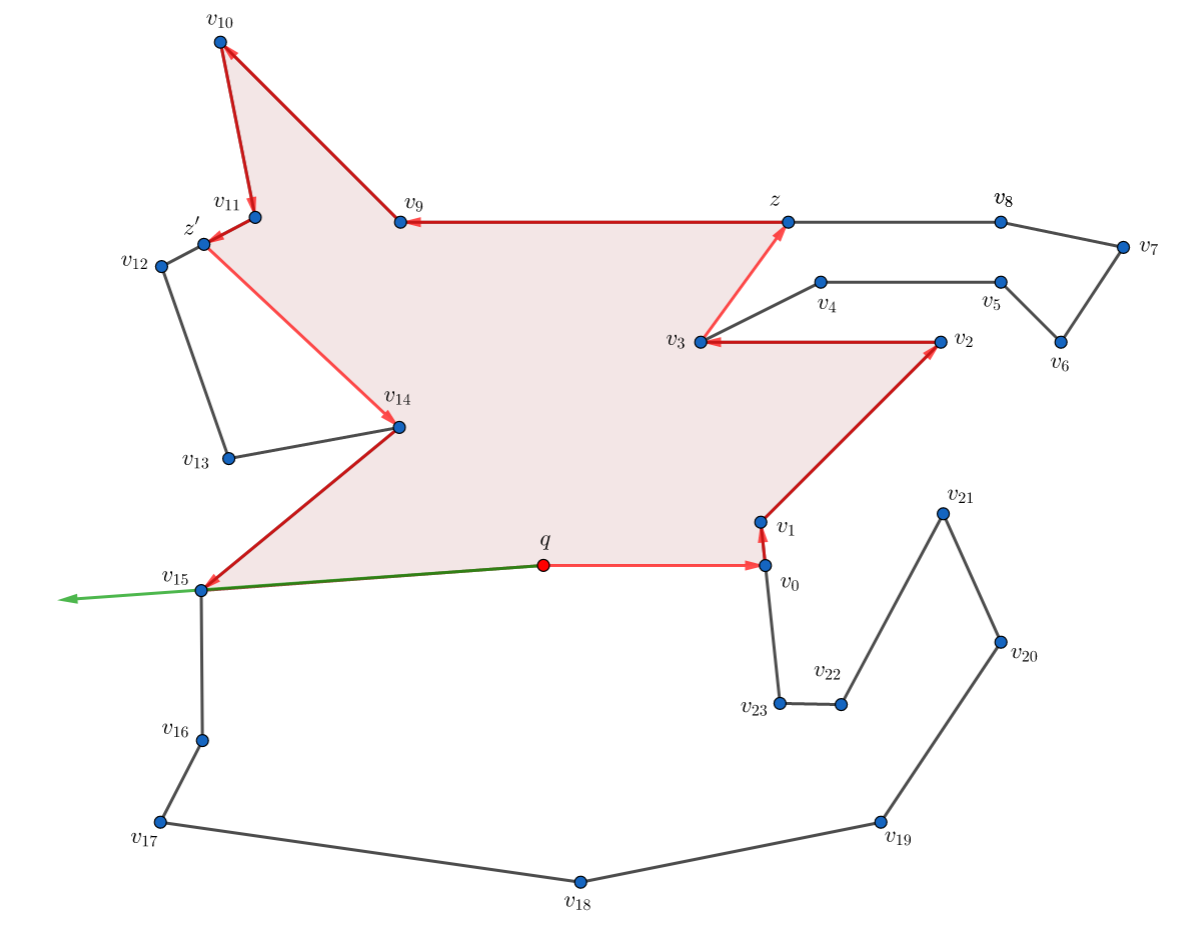
\includegraphics[width=0.70 \paperwidth]{images/Ejecucion/e20.png}
\end{frame}

\begin{frame}
  \centering 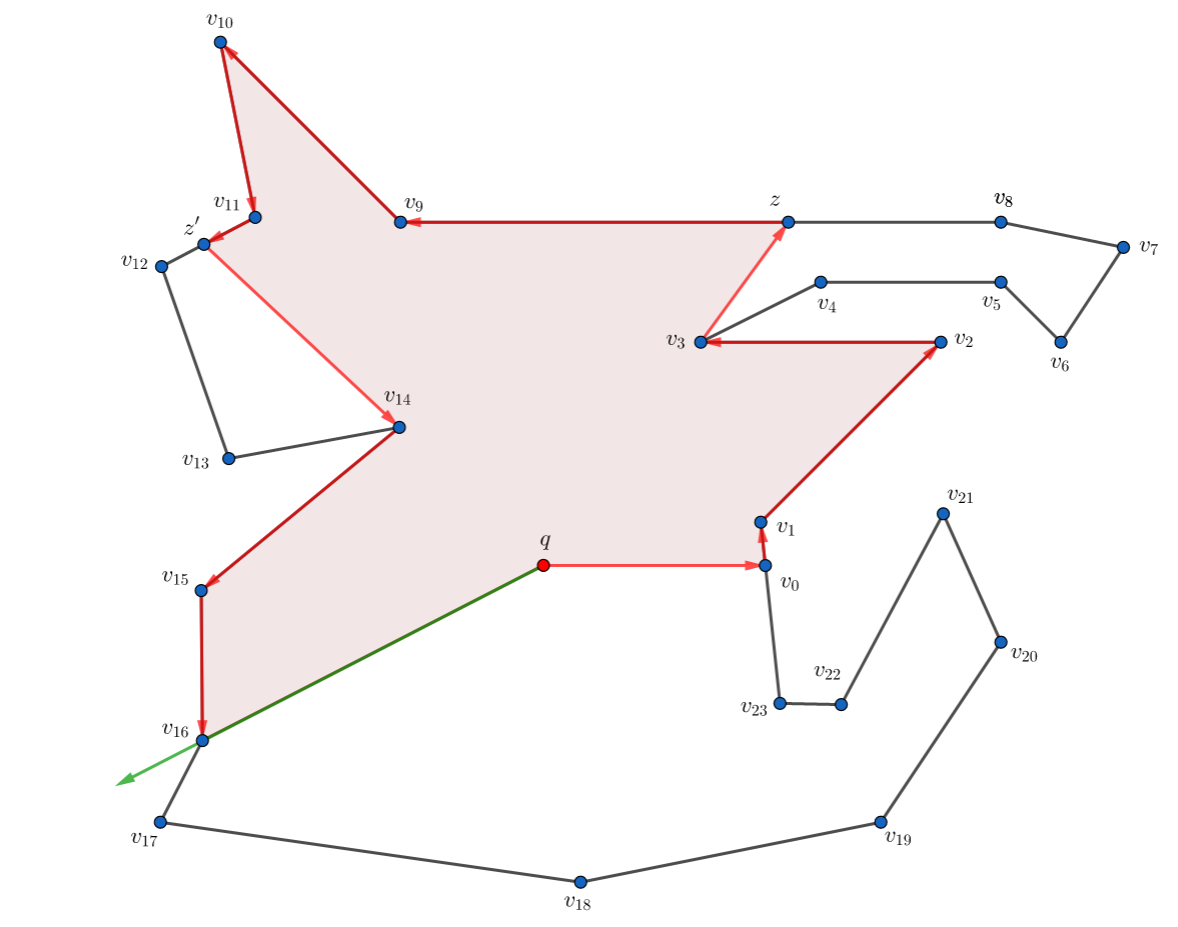
\includegraphics[width=0.70 \paperwidth]{images/Ejecucion/e21.png}
\end{frame}

\begin{frame}
  \centering 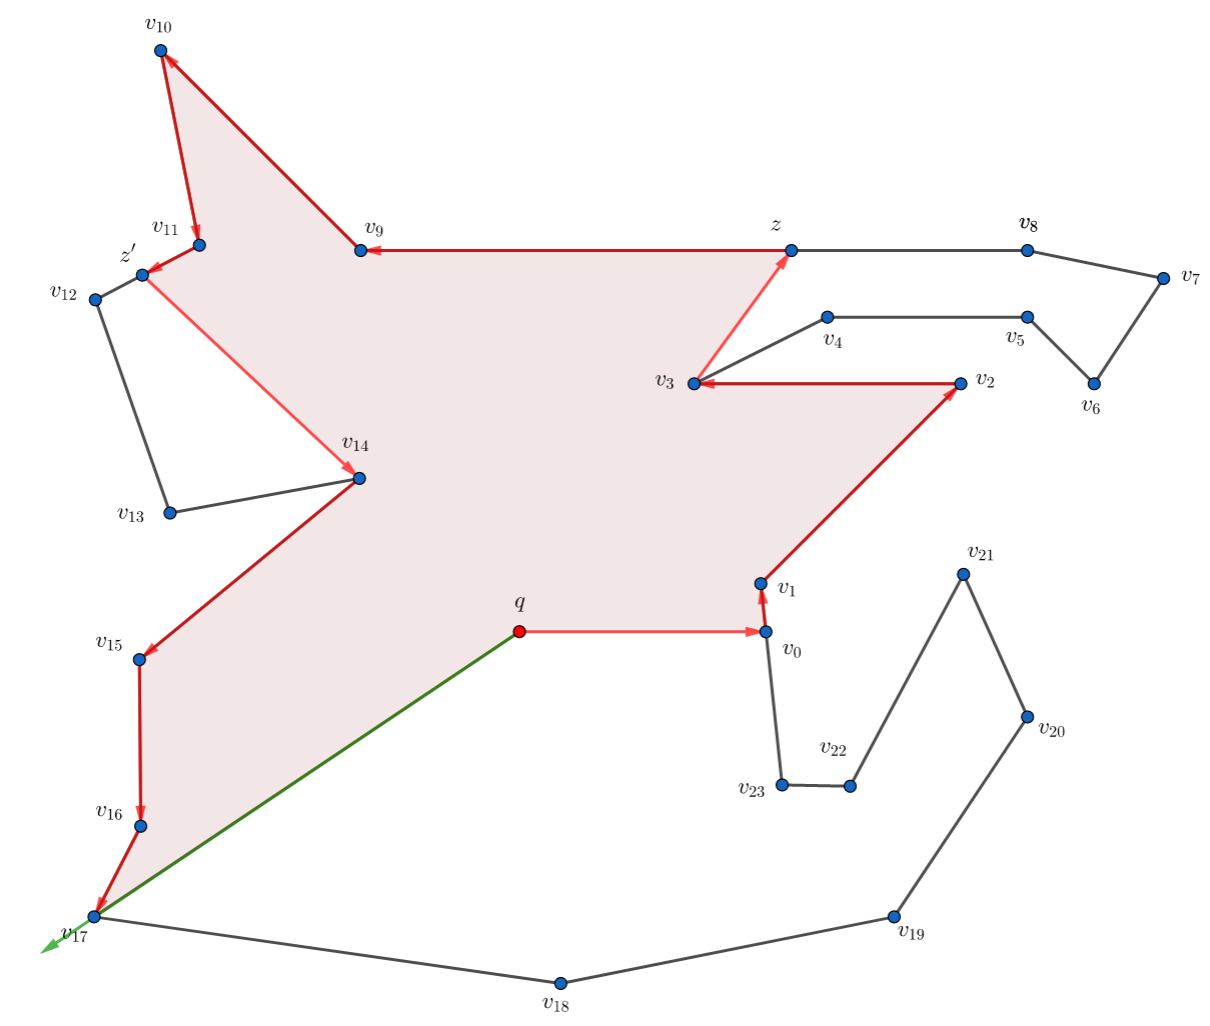
\includegraphics[width=0.70 \paperwidth]{images/Ejecucion/e22.png}
\end{frame}

\begin{frame}
  \centering 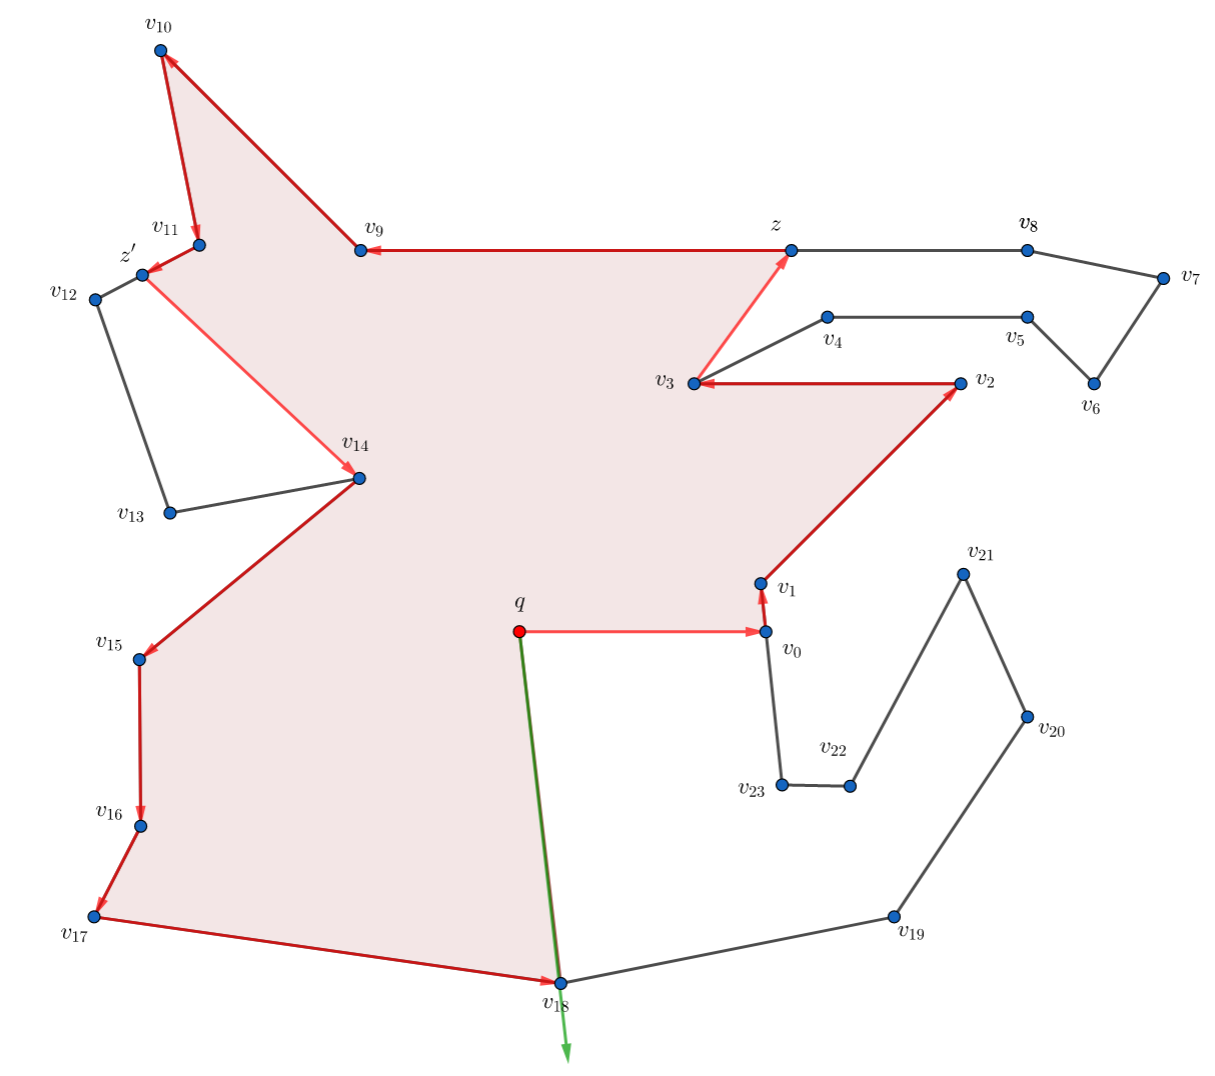
\includegraphics[width=0.70 \paperwidth]{images/Ejecucion/e23.png}
\end{frame}

\begin{frame}
  \centering 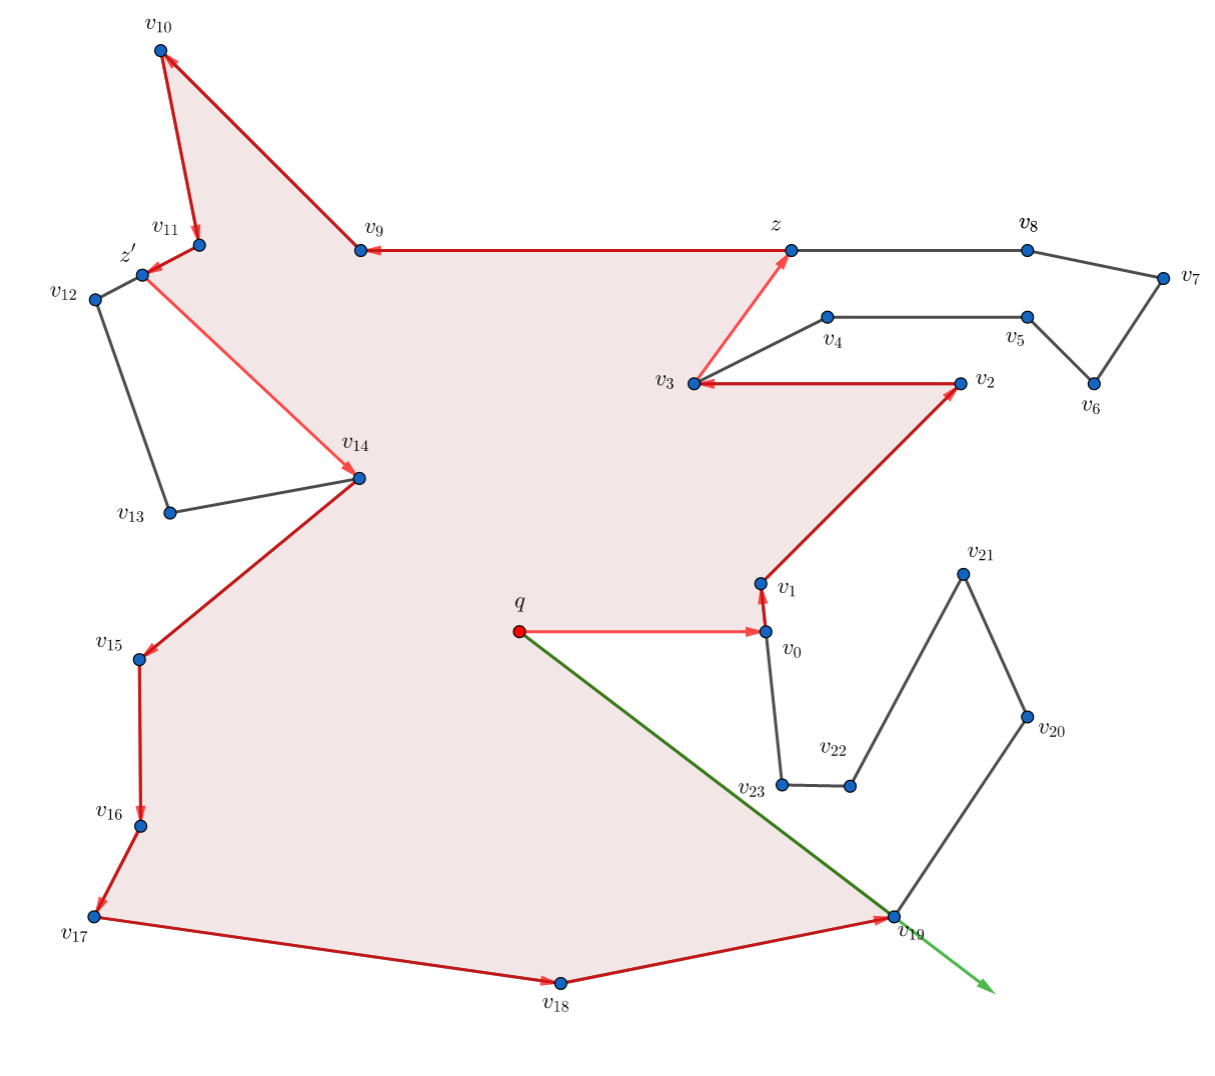
\includegraphics[width=0.70 \paperwidth]{images/Ejecucion/e24.png}
\end{frame}

\begin{frame}
  \centering 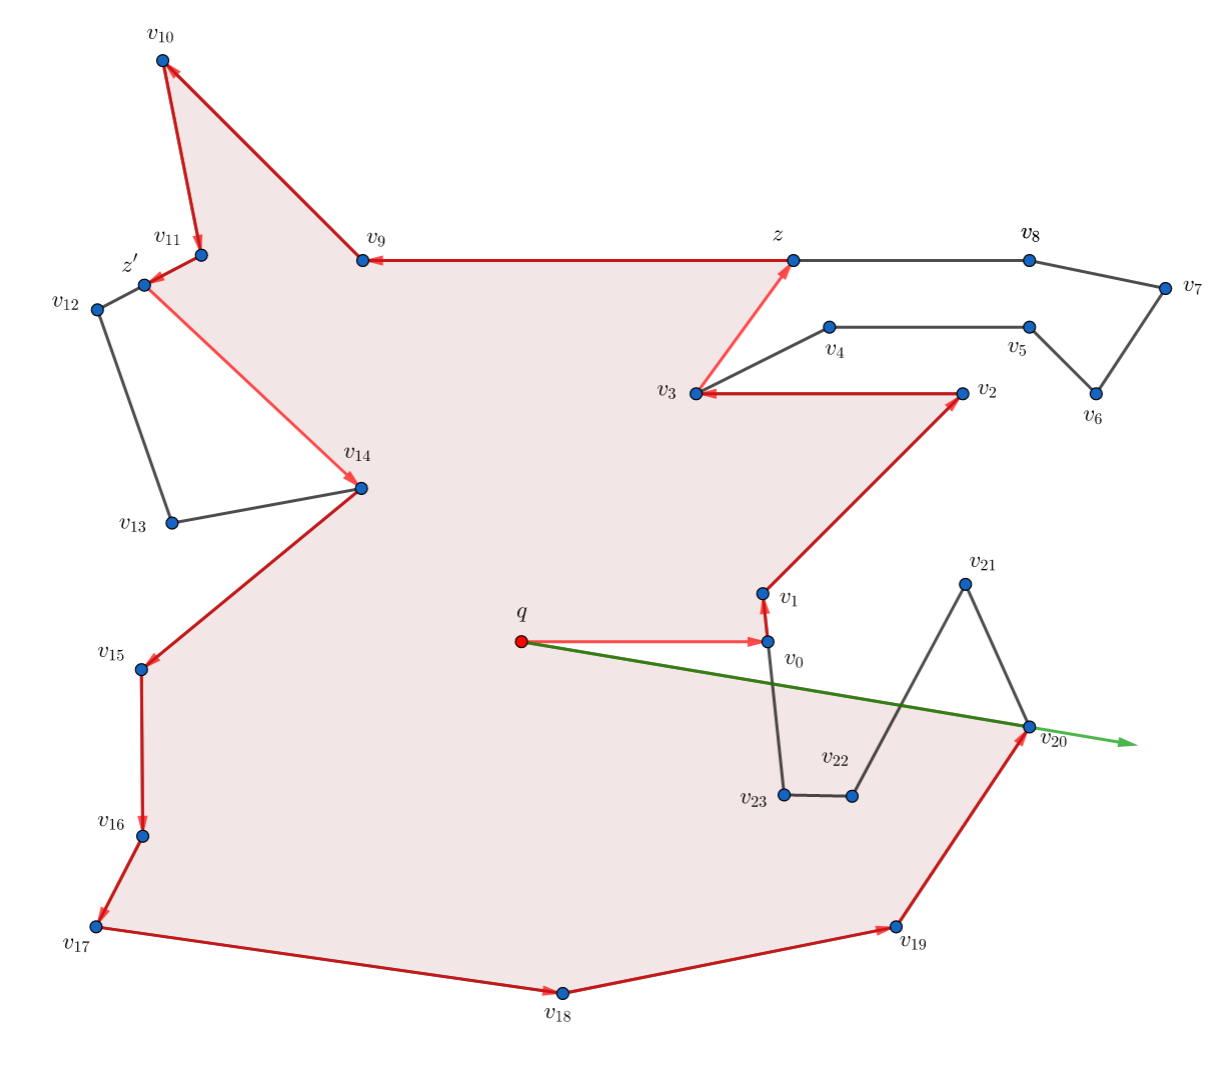
\includegraphics[width=0.70 \paperwidth]{images/Ejecucion/e25.png}
\end{frame}

\begin{frame}
  \centering 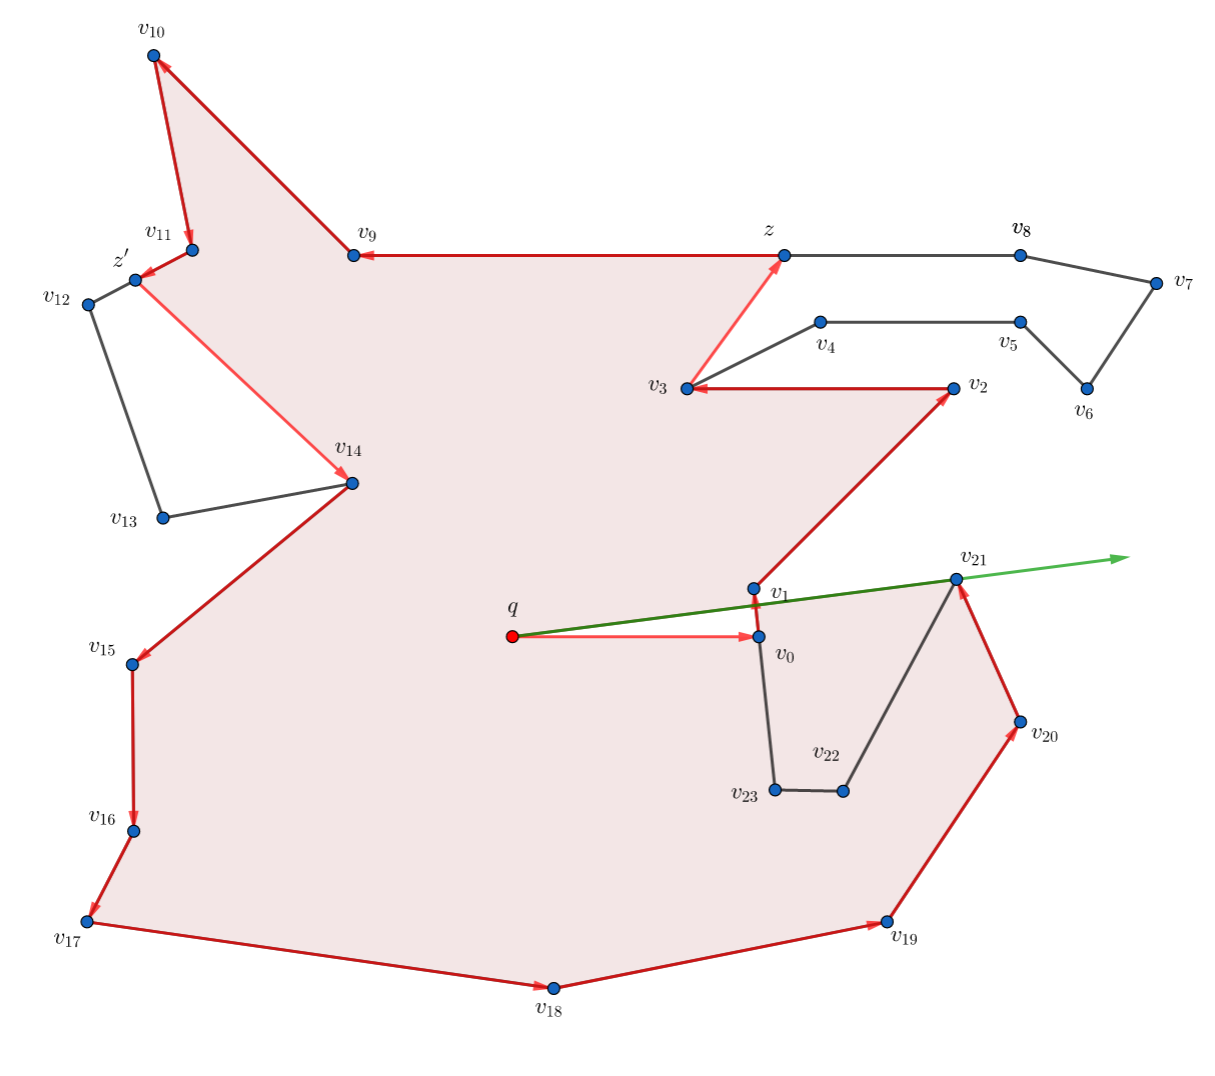
\includegraphics[width=0.70 \paperwidth]{images/Ejecucion/e26.png}
\end{frame}

\begin{frame}
  \centering 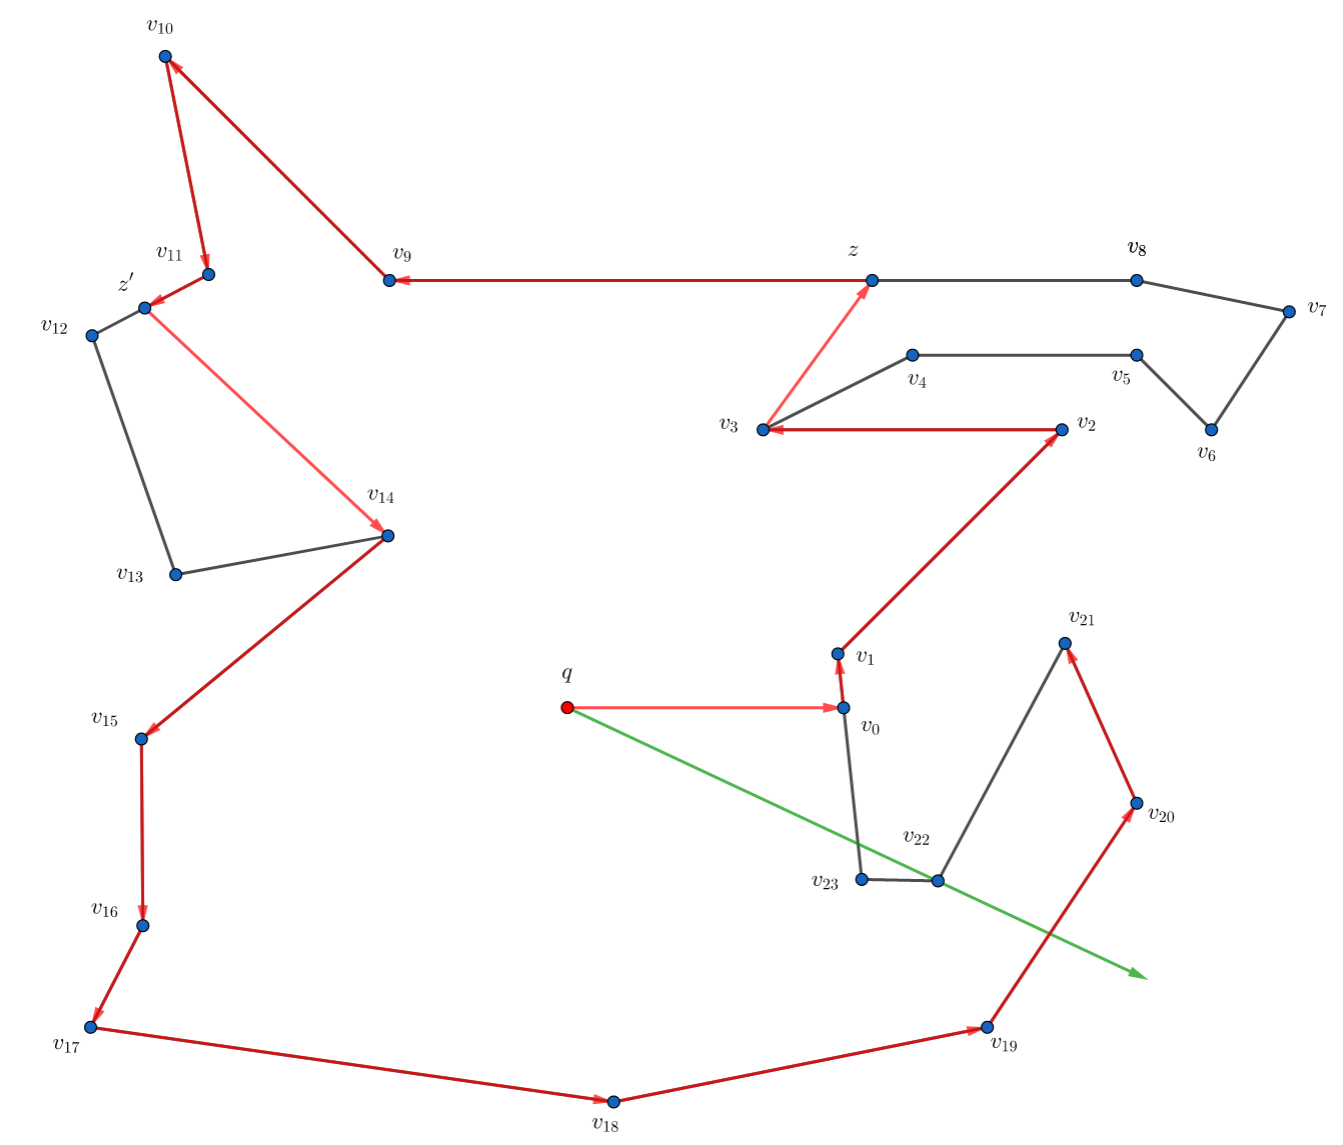
\includegraphics[width=0.70 \paperwidth]{images/Ejecucion/e27.png}
\end{frame}

\begin{frame}
  \centering 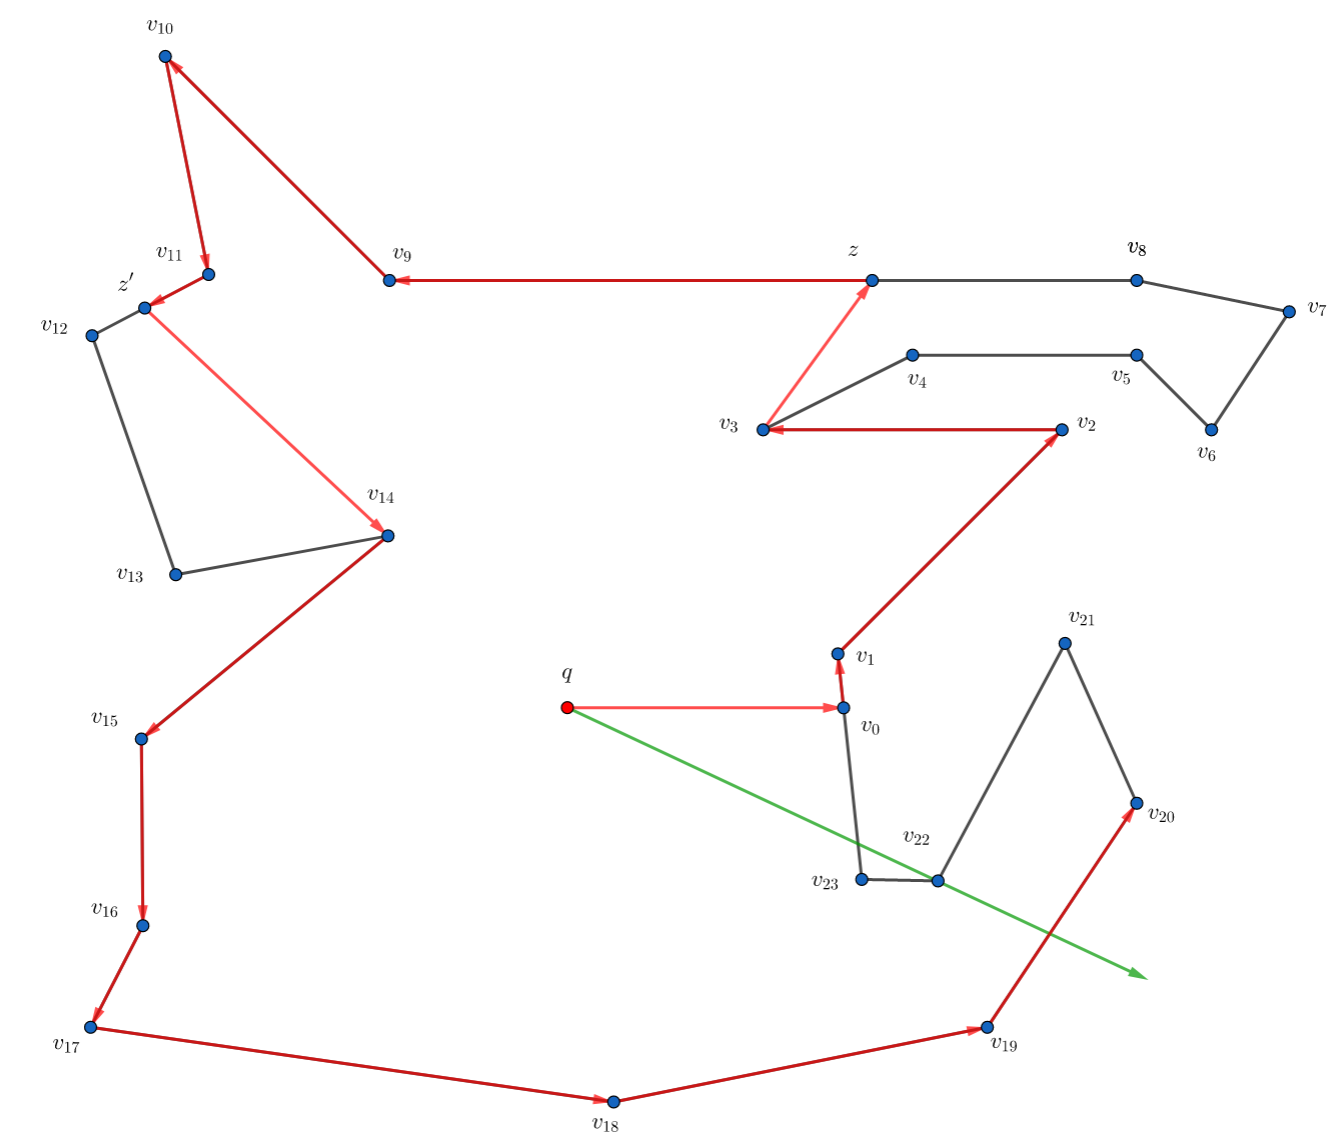
\includegraphics[width=0.70 \paperwidth]{images/Ejecucion/e28.png}
\end{frame}

\begin{frame}
  \centering 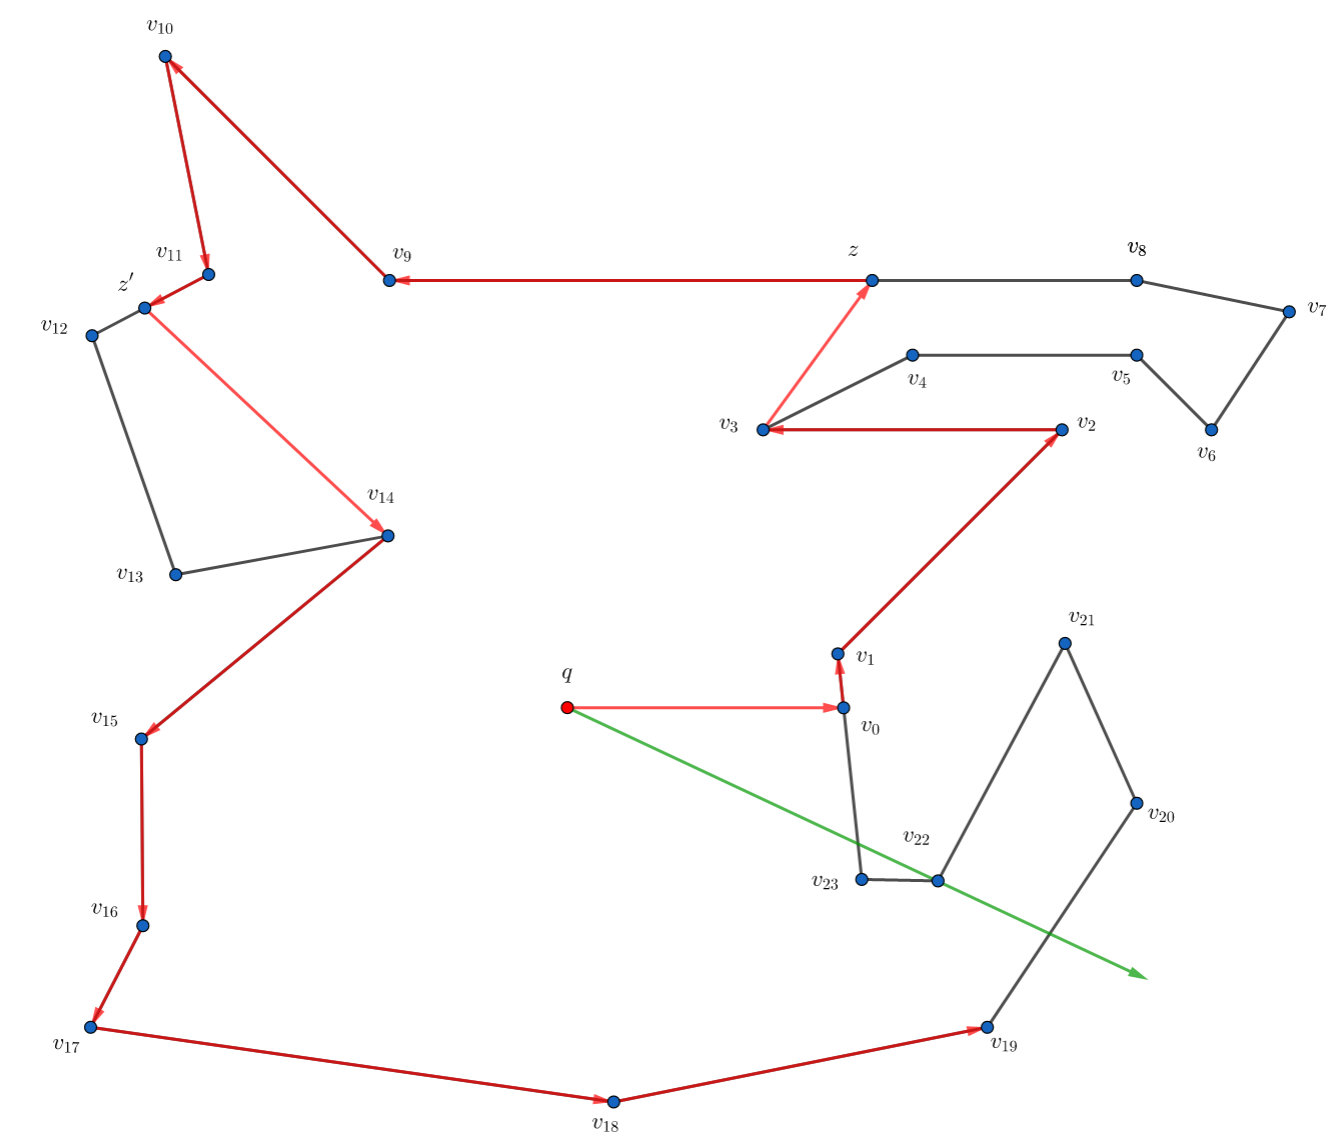
\includegraphics[width=0.70 \paperwidth]{images/Ejecucion/e29.png}
\end{frame}

\begin{frame}
  \centering 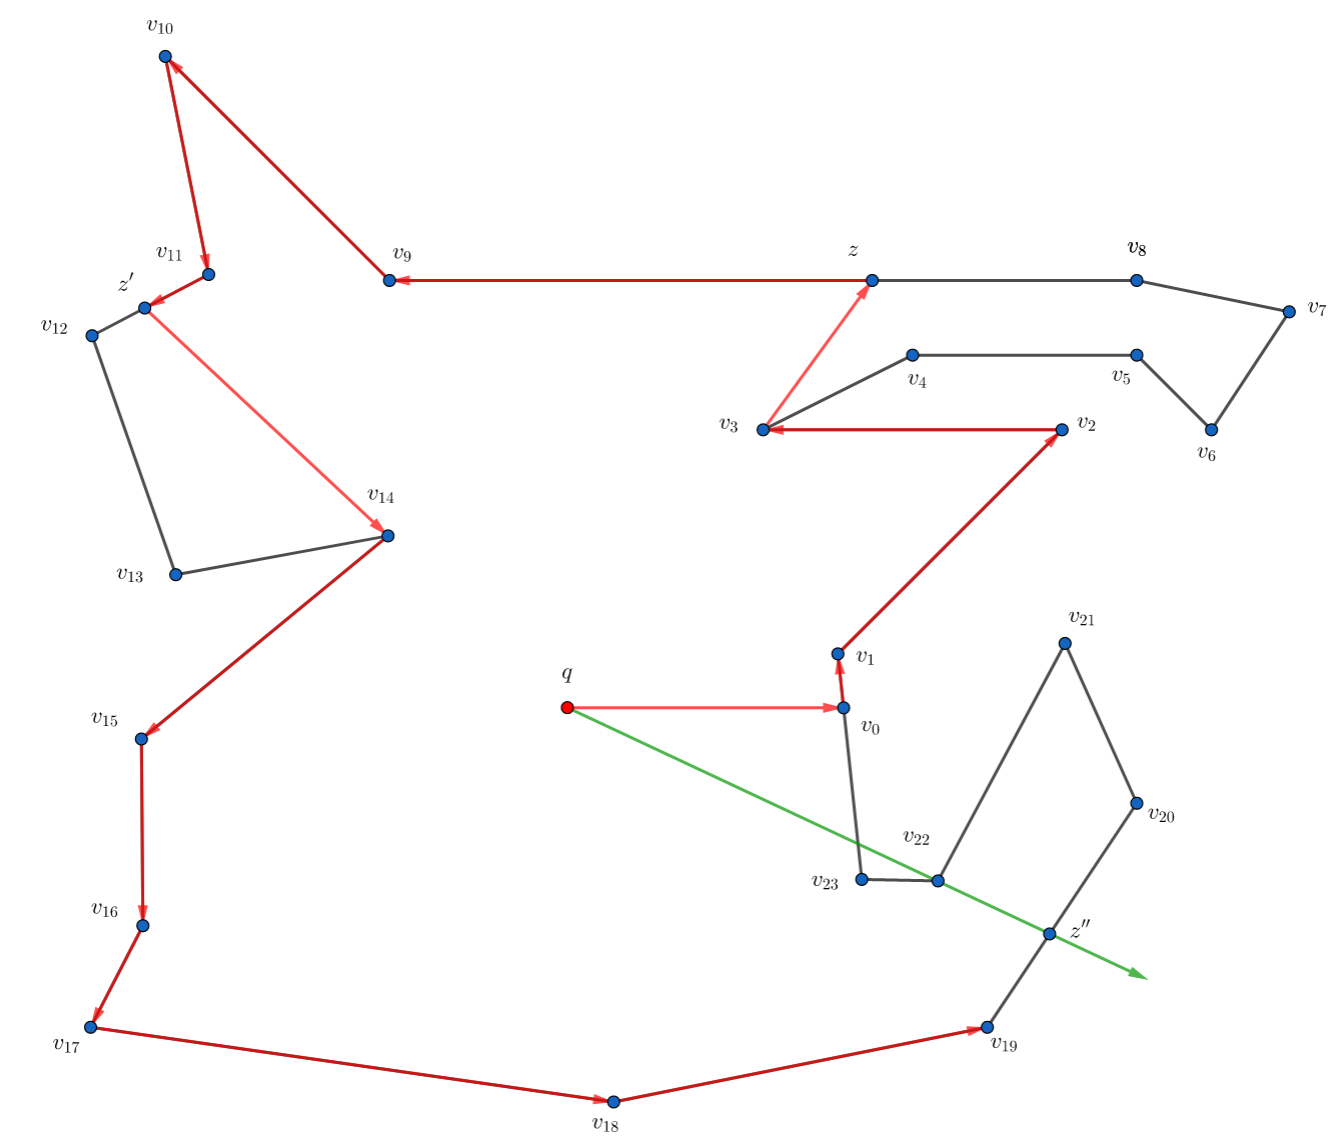
\includegraphics[width=0.70 \paperwidth]{images/Ejecucion/e30.png}
\end{frame}

\begin{frame}
  \centering 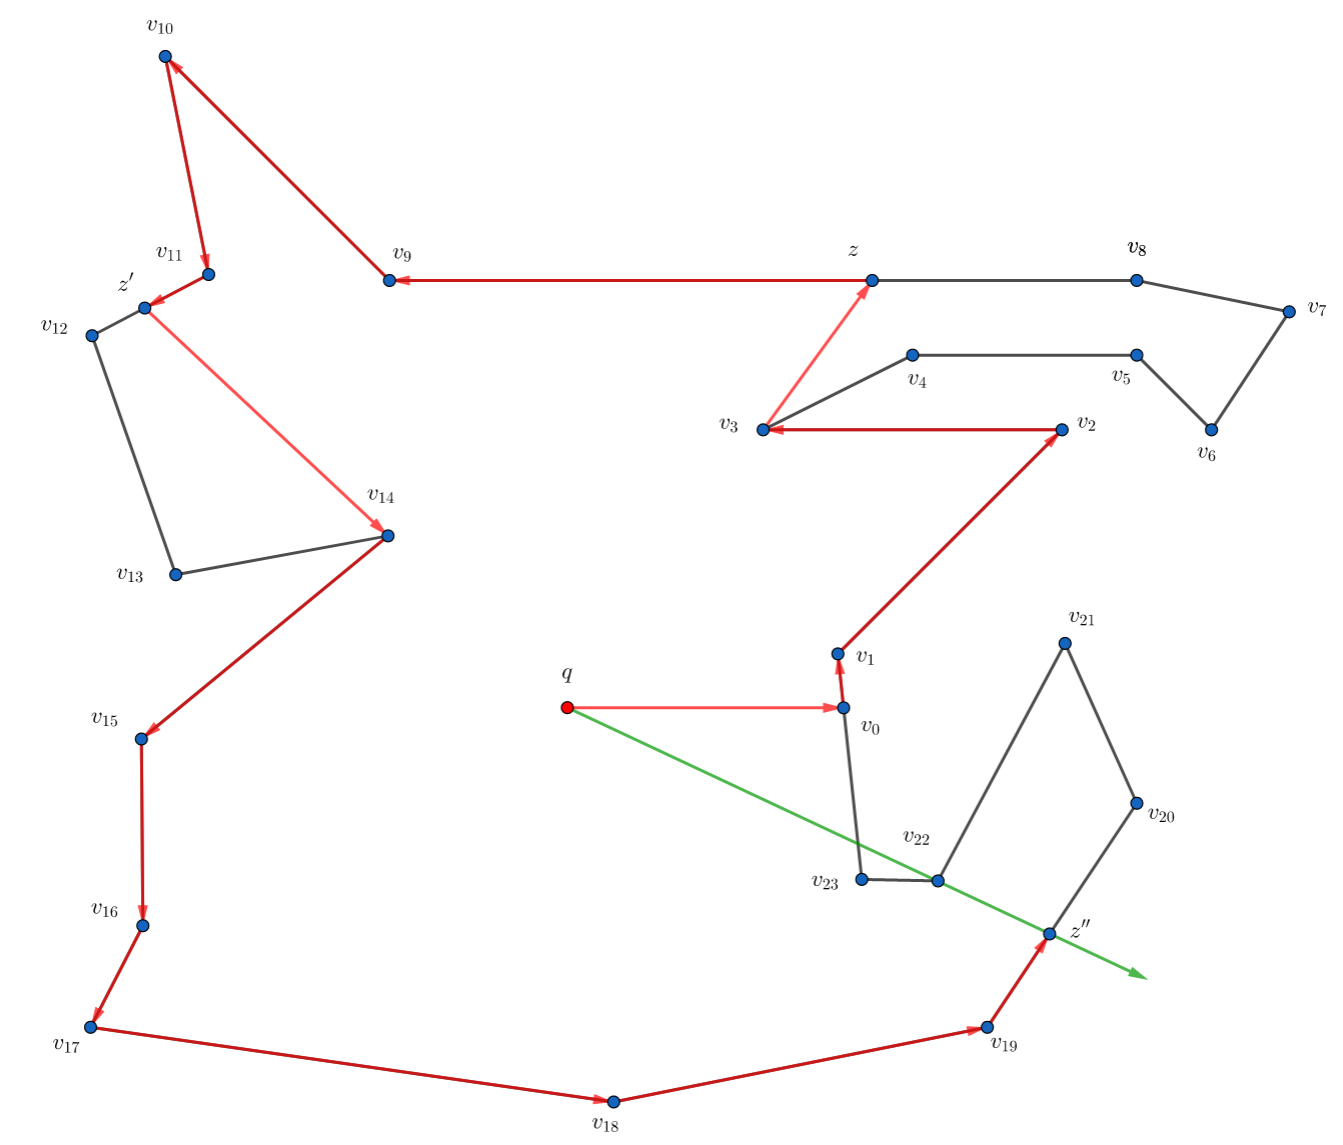
\includegraphics[width=0.70 \paperwidth]{images/Ejecucion/e31.png}
\end{frame}

\begin{frame}
  \centering 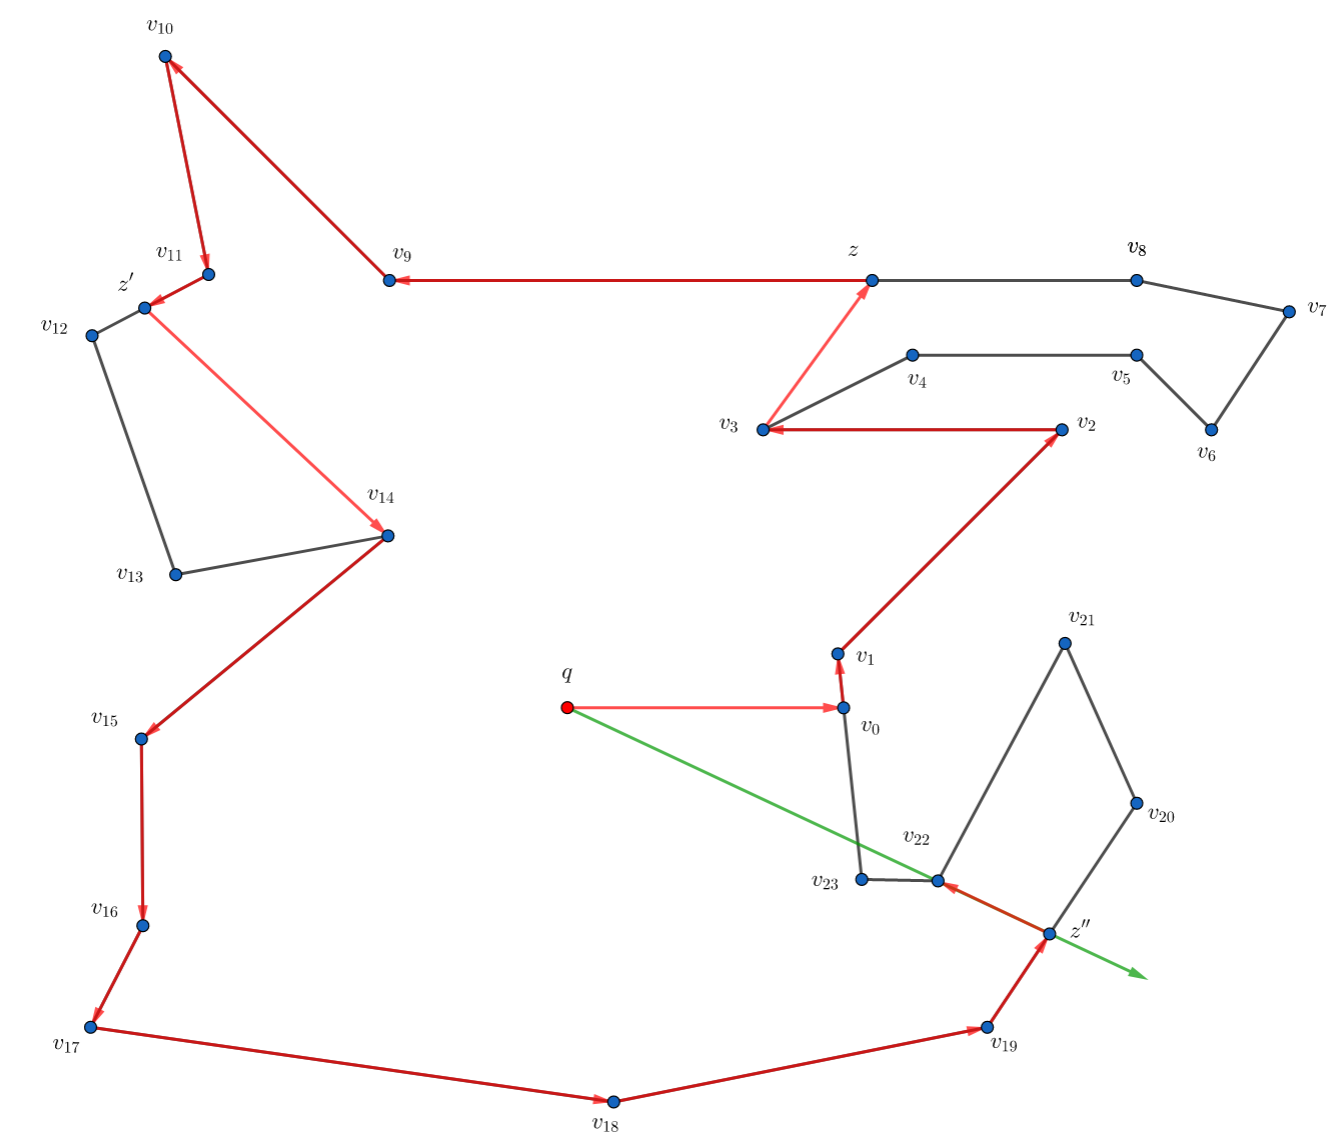
\includegraphics[width=0.70 \paperwidth]{images/Ejecucion/e32.png}
\end{frame}

\begin{frame}
  \centering 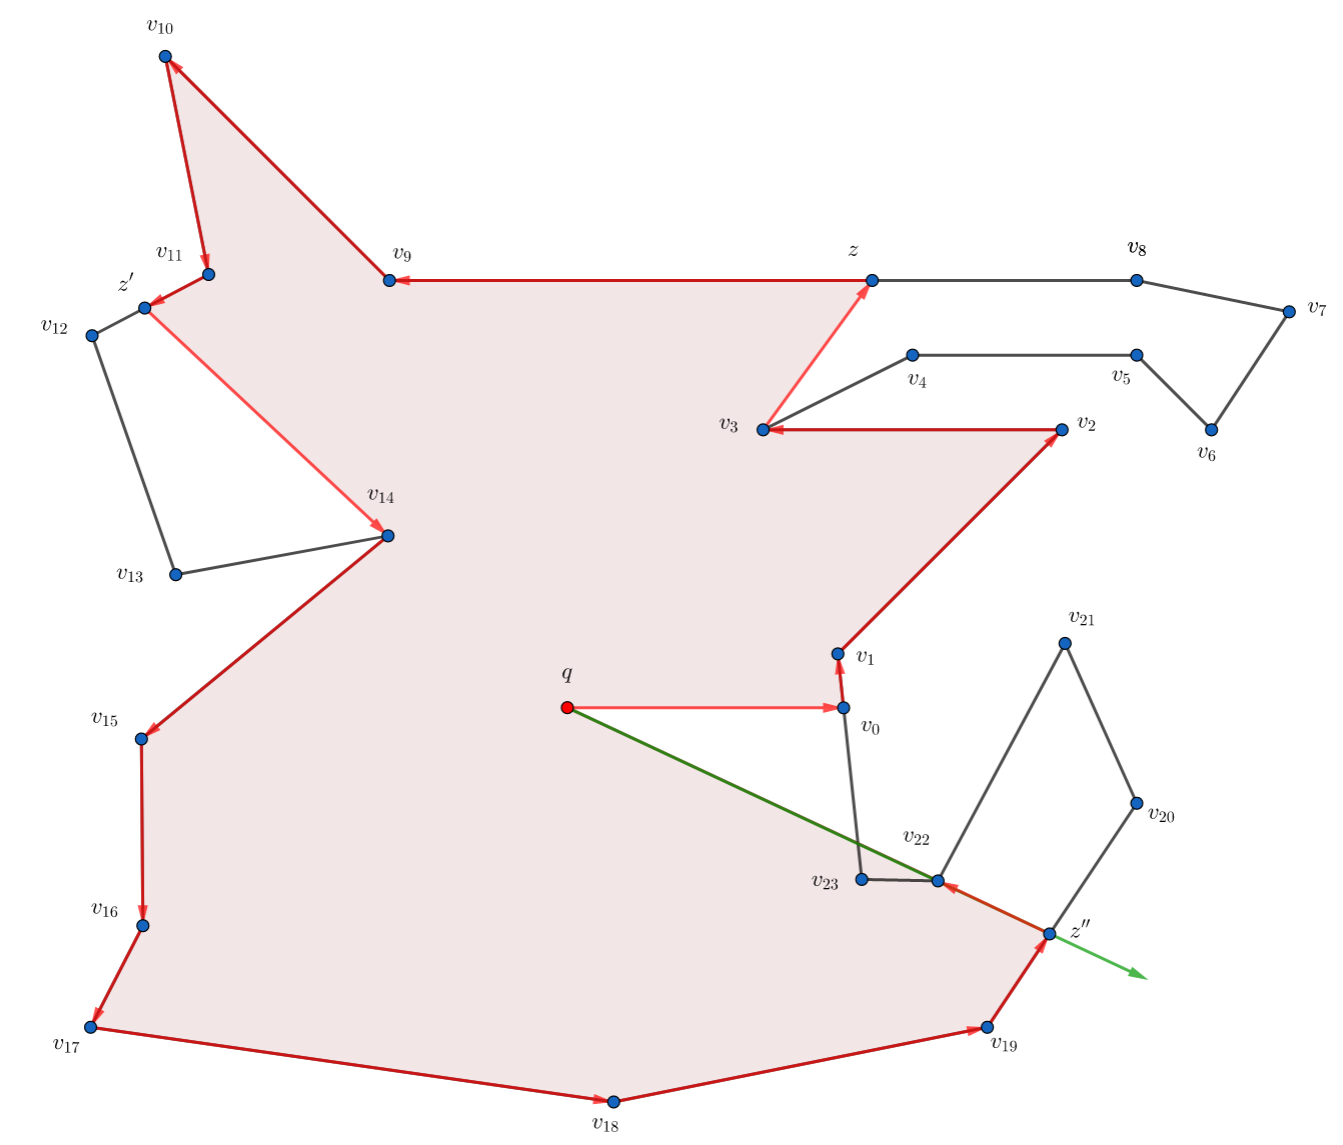
\includegraphics[width=0.70 \paperwidth]{images/Ejecucion/e33.png}
\end{frame}

\begin{frame}
  \centering 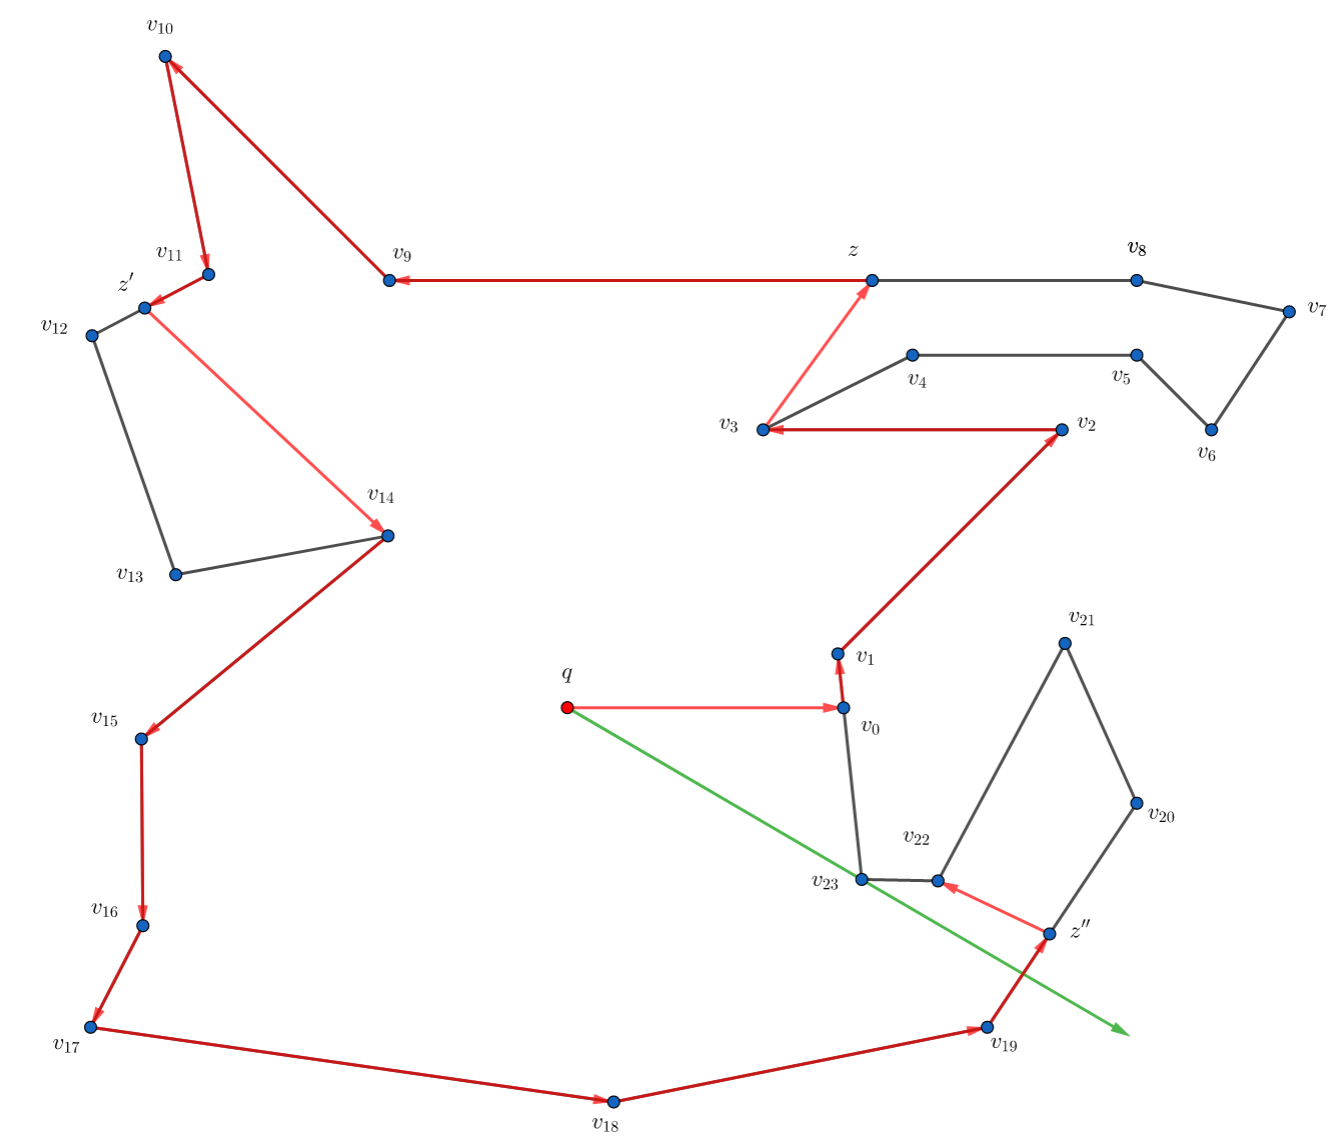
\includegraphics[width=0.70 \paperwidth]{images/Ejecucion/e34.png}
\end{frame}

\begin{frame}
  \centering 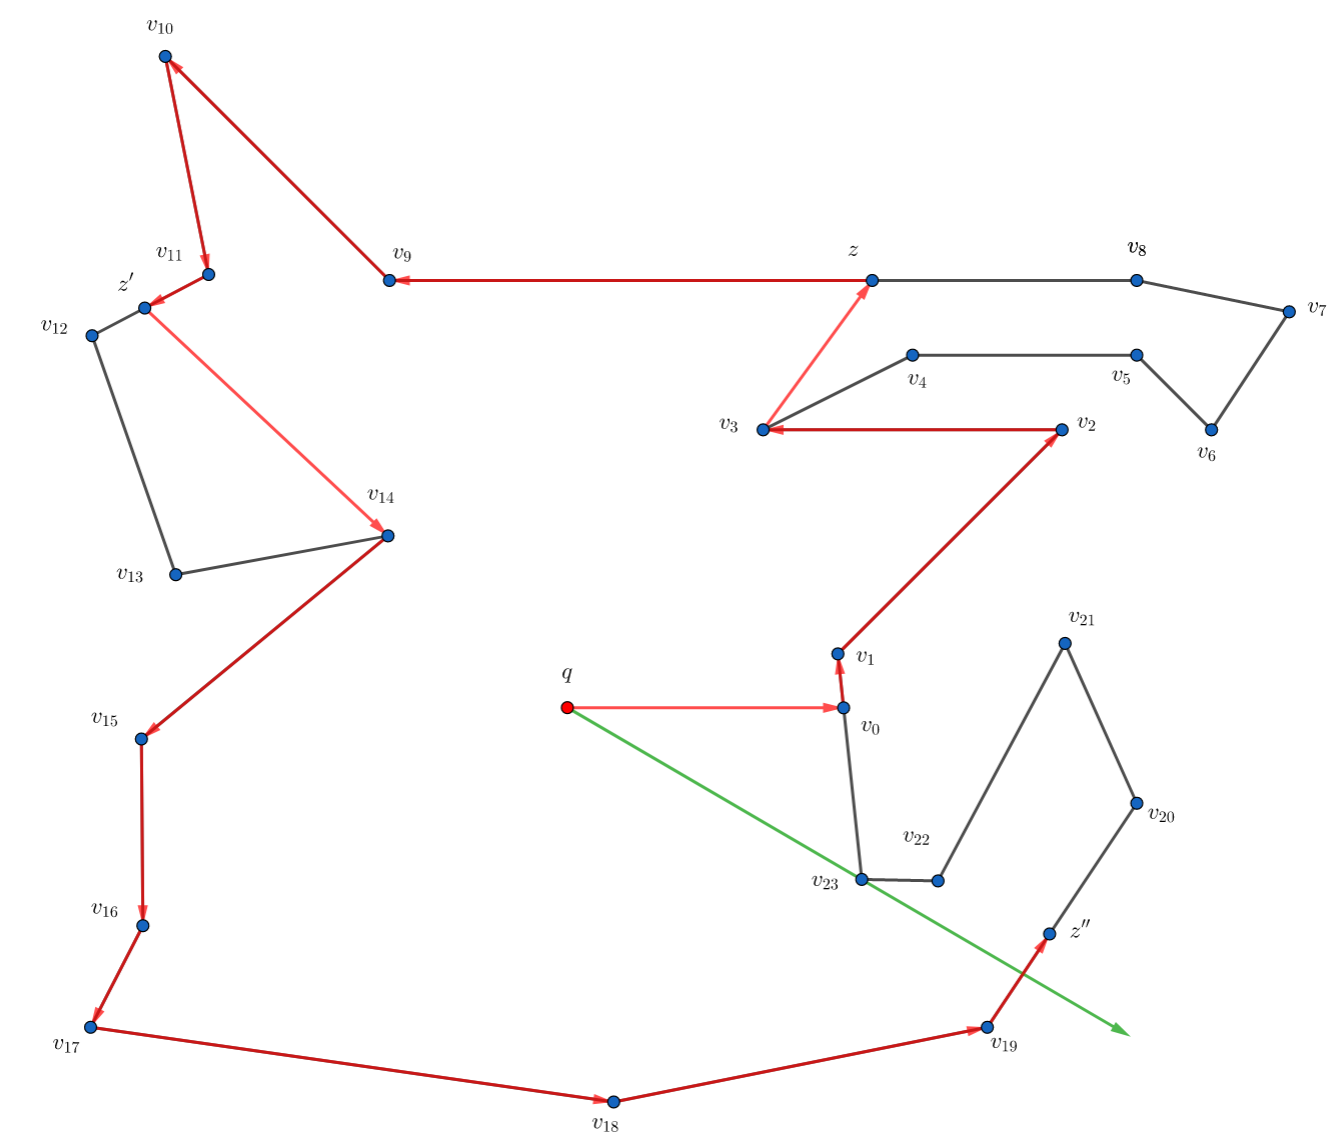
\includegraphics[width=0.70 \paperwidth]{images/Ejecucion/e35.png}
\end{frame}

\begin{frame}
  \centering \includegraphics[width=0.70 \paperwidth]{images/Ejecucion/e36.png}
\end{frame}

\begin{frame}
  \centering \includegraphics[width=0.70 \paperwidth]{images/Ejecucion/e37.png}
\end{frame}

\begin{frame}
  \centering \includegraphics[width=0.70 \paperwidth]{images/Ejecucion/e38.png}
\end{frame}

\begin{frame}
  \centering \includegraphics[width=0.70 \paperwidth]{images/Ejecucion/e39.png}
\end{frame}

\begin{frame}
  \centering \includegraphics[width=0.70 \paperwidth]{images/Ejecucion/e40.png}
\end{frame}

\begin{frame}
  \centering \includegraphics[width=0.70 \paperwidth]{images/Ejecucion/e41.png}
\end{frame}

\begin{frame}
  \centering \includegraphics[width=0.70 \paperwidth]{images/Ejecucion/e42.png}
\end{frame}

\subsection{Análisis de complejidad.}

\begin{frame}
  \frametitle{Análisis de complejidad.}
  \begin{enumerate}
  \item Encontrar el punto de intersección del primer rayo a partir de $q$ con la
    frontera del polígono simple $P$, lo realizamos en $\mathcal{O}(\log n)$ con una
    búsqueda en el orden del polígono.
  \item En cada paso de la iteración guardamos cada vértice una vez en una pila. Recorrer nuestro
    polígono nos toma $\mathcal{O}(n)$.
  \item Encontrar la intersección del rayo con la arista incidente nos toma $\mathcal{O}(1)$, pues
    es suficiente hacer pop en la pila usada.
  \item Verificar en cada iteración la dirección del vértice siguiente lo podemos realizar en $\mathcal{O}(1)$.
  \end{enumerate}
\end{frame}

\subsection{Casos especiales.}

\begin{frame}
  \frametitle{Casos especiales.}
  Existen dos casos espciales para encontrar $V(q)$ de $P$, estos son
  \begin{itemize}
  \item $q$ está fuera de $P$ y se encuentra dentro de la envolvente convexa del polígono simple $P$.
  \item $q$ está fuera de $P$ y se encuentra fuera de la envolvente convexa del polígono simple $P$.
  \end{itemize}
\end{frame}

\begin{frame}
  \frametitle{Caso 1.}
  \centering \includegraphics[width=0.50 \paperwidth]{images/CasosQExterno/P.png}
\end{frame}

\begin{frame}
  \frametitle{Caso 1.}
  \centering \includegraphics[width=0.50 \paperwidth]{images/CasosQExterno/P01.png}
\end{frame}

\begin{frame}
  \frametitle{Caso 1.}
  \centering \includegraphics[width=0.50 \paperwidth]{images/CasosQExterno/P02.png}
\end{frame}

\begin{frame}
  \frametitle{Caso 1.}
  \centering \includegraphics[width=0.50 \paperwidth]{images/CasosQExterno/P03.png}
\end{frame}

\begin{frame}
  \frametitle{Caso 1.}
  \centering \includegraphics[width=0.50 \paperwidth]{images/CasosQExterno/P04.png}
\end{frame}

\begin{frame}
  \frametitle{Caso 1.}
  \centering \includegraphics[width=0.50 \paperwidth]{images/CasosQExterno/P05.png}
\end{frame}

\begin{frame}
  \frametitle{Caso 2.}
  \centering \includegraphics[width=0.50 \paperwidth]{images/CasosQExterno/P.png}
\end{frame}

\begin{frame}
  \frametitle{Caso 2.}
  \centering \includegraphics[width=0.50 \paperwidth]{images/CasosQExterno/P01.png}
\end{frame}

\begin{frame}
  \frametitle{Caso 2.}
  \centering \includegraphics[width=0.50 \paperwidth]{images/CasosQExterno/P02F.png}
\end{frame}

\begin{frame}
  \frametitle{Caso 2.}
  \centering \includegraphics[width=0.45 \paperwidth]{images/CasosQExterno/P03F.png}
\end{frame}

\begin{frame}
  \frametitle{Caso 2.}
  \centering \includegraphics[width=0.45 \paperwidth]{images/CasosQExterno/P04F.png}
\end{frame}


\begin{frame}
  \frametitle{Análisis de complejidad.}
  \begin{enumerate}
  \item Encontrar la envolvente convexa de $P$ por medio del algoritmo de Graham-Jao nos toma $\mathcal{O}(n)$.
  \item Encontrar $q'$ o en su defecto las tangentes a $P$ nos toma $\mathcal{O}(\log n)$.
  \item Unir las fronteras encontradas nos toma a lo más $\mathcal{O}(n)$.
  \end{enumerate}
\end{frame}


%%%%%%%%%%%%%%%%%%%%%%%%%%%%%%%%%%%%%%%% Última diapo xD
\section{Fin.} %%Título de la sección (Opcional)
\begin{frame}{Gracias}
  \begin{figure}
    \centering
    \includegraphics[width=.35 \paperwidth]{./images/Agradecimientos.jpg}
    %\caption*{.}
  \end{figure}
\end{frame}

\end{document}
